% SETUP
\documentclass[11pt]{article}
\linespread{1.25}
\usepackage[utf8]{inputenc}
\usepackage{graphicx, amsmath, array, graphics, amssymb, epsfig, psfrag, geometry, alltt, subfiles, blindtext, enumitem,float,pdfpages,multicol}
\DeclareMathOperator{\sinc}{sinc}
\usepackage[export]{adjustbox}
\usepackage{fancyhdr}
\usepackage{array}
\usepackage{hyperref}
%%%%%%%%%%%%%%  code listing
\usepackage{listings}
\usepackage{color} %red, green, blue, yellow, cyan, magenta, black, white
\definecolor{mygreen}{RGB}{2,94,33} % color values Red, Green, Blue
\definecolor{mylilas}{RGB}{170,55,241}

\lstset{language=Matlab,%
    %basicstyle=\color{red},
    breaklines=true,%
    morekeywords={matlab2tikz},
    keywordstyle=\color{blue},%
    morekeywords=[2]{1}, keywordstyle=[2]{\color{black}},
    identifierstyle=\color{black},%
    stringstyle=\color{mylilas},
    commentstyle=\color{mygreen},%
    showstringspaces=false,%without this there will be a symbol in the places where there is a space
    numbers=left,%
    numberstyle={\tiny \color{black}},% size of the numbers
    numbersep=9pt, % this defines how far the numbers are from the text
    emph=[1]{for,end,break},emphstyle=[1]\color{black}, %some words to emphasise
    %emph=[2]{word1,word2}, emphstyle=[2]{style},    
}
%%%%%%%%%%%%%%%%


\geometry{a4paper, top = 20mm, bottom = 20mm, left = 15mm, right = 15mm}

% Headers
\pagestyle{fancy}
\fancyhf{}
\chead{ELEN90057 Communication Systems - Workshop 3 Report}
\cfoot{\thepage}

\begin{document}
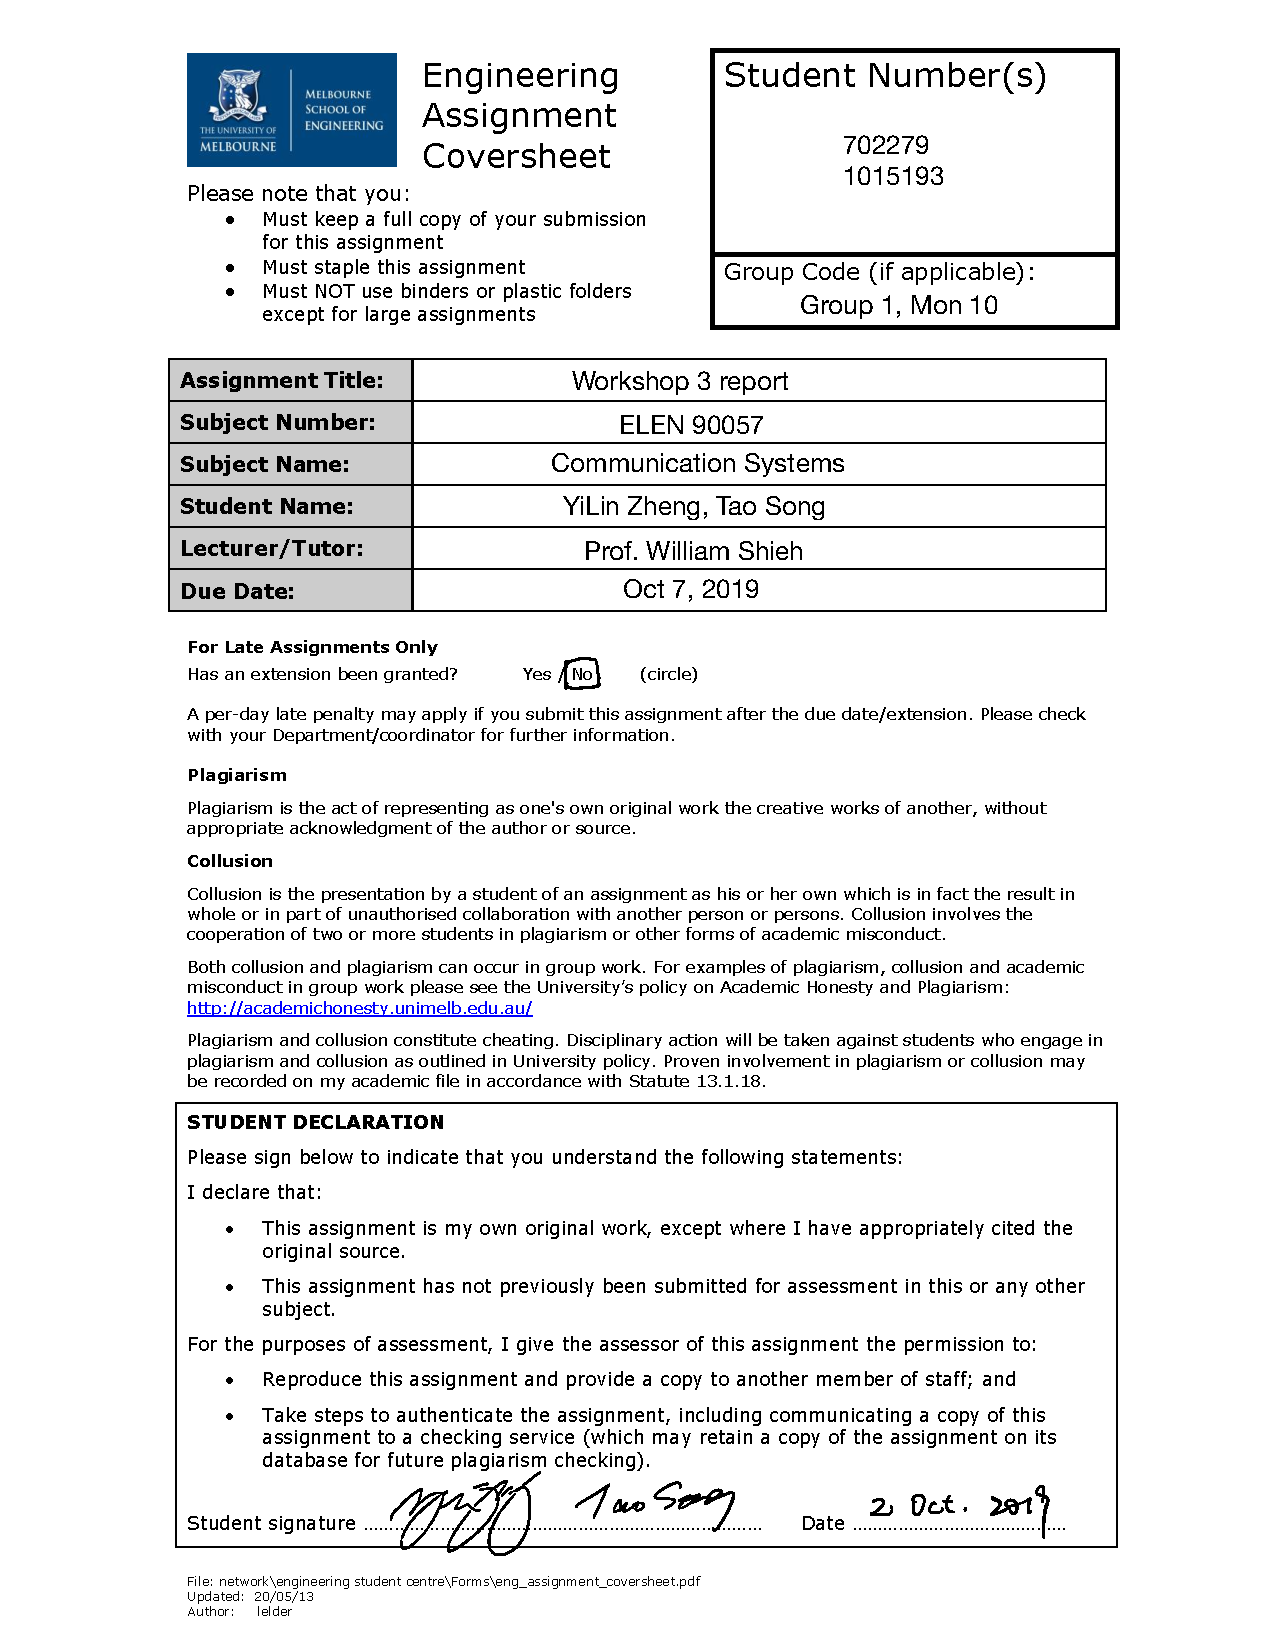
\includepdf{coverpage3.pdf}
% Title
\begin{center}
\textbf{\Large{Workshop 3}}\\
Group 1: Tao Song [1015193], YiLin Inez Zheng [702279], \\
Workshop: Monday 10:00am - 12:00pm (Shalanika, Bigi), Due: 07/10/19  
\end{center}

% Q1, I edited some delta things! Please check. %%%%%%% checked
% Q2, Ok.  %%%%%%%  checked
% Q3, May have changed some wording. Calcs are all ok. %%%%%%% checked
% Q4, Wrote more and put in Carson's Bandwidths. I don't remember what this one was so put in some random value. Please check explanations for 3.3?

% I have added some arguments for Carson's rule on bandwidth. 3.3 and the entire Q4 looks good to me. btw i think there is a typo on lab instruction: i think it should be carson's rule. %%% yea have changed to carson's

% Q5, I added in calculations for 2.5us? I'm not sure why I did that... can't remember... we can delete it if it doesn't make sense...  %%%%%% lets just leave it like that, i dont have anything better to demonstrate. %%% ok

% Q6 please see my comments on b) and d). 
%%%%% I have added something in b), please see if this makes sense to you. as for d), let's just leave it like that.

%%%%%%%%%%% So far, this report looks good to me for submission.  

% Configs added
%%%%%%%%% thanks, good drawing

\section*{Question 1}
\begin{enumerate}[label=(\alph*)]
\item When we want to have SSB modulation, we use a 90 degree phase shifter (quadrature phase splitter) to take an input signal $x(t)$ and generate two output signals with 90 degrees phase difference. The two output signals can be simply expressed as $x(t)$ and $\tilde{x}(t)$. The two output signals from phase splitter will then multiply with carrier cosine and sine waves to create the SSB signal which consists of two DSBSC-like signals: $m(t)\cos(2\pi f_c t)$ and $\tilde{x}(t)\sin(2\pi f_c t)$. The math expression of the SSB signal $s(t)$ is given by Equation \ref{eq:SSB}. The carrier signals used in this have been scaled down in amplitude by $\frac{A_c}{2}$ to give a demodulated amplitude similar to that of a DSBSC signal as the SSB signal will have an amplitude doubling effect. 
\begin{equation}\label{eq:SSB}
    s(t)=\frac{A_c}{2} \biggr (x(t)\cos(2\pi f_c t) \pm \tilde{x}(t)\sin(2\pi f_c t) \biggr)
\end{equation}
Now, from the question we have $m(t)$ that is approximately equal to $x(t)$. The SSB signal $s(t)$ in time domain can be found as:
\begin{align*}
    s(t)=\frac{A_c}{2} \biggr (m(t)\cos(2\pi f_c t) \pm \tilde{m}(t)\sin(2\pi f_c t) \biggr)
\end{align*}
Substituting in $m(t) = \frac{1}{2}\cos(2\pi f_m t)+ \cos(2\pi 2f_m t)$ and $\tilde{m(t)} = \frac{1}{2}\sin(2\pi f_m t)+ \sin(2\pi 2f_m t)$ we have,
\begin{align*}
    s(t) &= \frac{A_c}{2} \biggr( \frac{1}{2}\cos(2\pi f_m t)\cos(2\pi f_c t) + \cos(2\pi 2f_m t) \cos(2\pi f_c t) \biggr)\\
    \hspace{1cm} &\pm \frac{A_c}{2} \biggr( \frac{1}{2}\sin(2\pi f_m t) \sin(2\pi f_c t) + \sin(2\pi 2f_m t) \sin(2\pi f_c t) \biggr)\\
    &= \frac{A_c}{4}\cos \bigg( 2\pi (f_c \mp f_m)t \bigg) + \frac{A_c}{2} \cos \bigg( 2\pi (f_c \mp 2 f_m)t \bigg)
\end{align*}
%\begin{align*}
%    m(t)=\frac{1}{2}\cos(2\pi f_m t)+ \cos(2\pi 2f_m t) \\
%    \tilde{m(t)}=\frac{1}{2}\sin(2\pi f_m t)+ \sin(2\pi 2f_m t)
%\end{align*}
Now, the Fourier transform gives, 
\begin{align*}
    S(f)=\frac{A_c}{8} \bigg[ \delta(f - (f_c \mp f_m)) + \delta(f + (f_c \mp f_m)) \bigg] + \frac{A_c}{4} \bigg[ \delta(f - (f_c \mp 2f_m)) + \delta(f + (f_c \mp 2f_m)) \bigg]
\end{align*}
%Prior to taking Fourier transform, we will need to re-write $s(t)$ of SSB as: 
%\begin{align*}
%    s(t)=\frac{A_c}{2} \biggr (m(t)\frac{e^{j2\pi f_c t}+e^{-j2\pi f_c t}}{2} \pm %\tilde{m}(t)\frac{e^{j2\pi f_c t} -e^{-j2\pi f_c t}}{j2} \biggr)
%\end{align*}
%where $A_c$ is the magnitude of carrier, we also rewrite the messages as:
%\begin{align*}
%    m(t)=\frac{1}{2}\frac{e^{j2\pi f_m t}+e^{-j2\pi f_m t}}{2}+\frac{e^{j2\pi 2f_m t}+e^{-j2\pi 2f_m t}}{2} \\
%    \tilde{m(t)}=\frac{1}{2}\frac{e^{j2\pi f_m t}-e^{-j2\pi f_m t}}{j2}+\frac{e^{j2\pi 2f_m t}+e^{-j2\pi 2f_m t}}{j2}
%\end{align*}
\textit{Note that the $\pm$ sign in $s(t)$ attributes to the respective USSB and LSSB Fourier transform peaks. Due to the simplification in $s(t)$ the choice of $+$ or $-$ has an inverse effect shown in the FFT's $\mp$.}\\

When we take $-$ sign from $s(t)$ in Eq.\ref{eq:SSB} or $+$ in the $\pm$ in the Fourier transform we have,
\begin{align*}
     S_+(f)=\frac{A_c}{8} \bigg[ \delta(f - (f_c + f_m)) + \delta(f + (f_c + f_m)) \bigg] + \frac{A_c}{4} \bigg[ \delta(f - (f_c + 2f_m)) + \delta(f + (f_c + 2f_m)) \bigg]
\end{align*}
This yields 4 frequency components which are all in upper sideband (USSB):
\begin{multicols}{4}
\begin{itemize}
    \item $f_1=f_c+f_m$
    \item $f_2=-(f_c+f_m)$
    \item $f_3=f_c+2f_m$
    \item $f_4=-(f_c+2f_m)$
\end{itemize}
\end{multicols}
When only considering the positive frequencies we will only see 2 peaks at $f_1$ and $f_3$, which are 102kHz and 104kHz when using a carrier frequency of 100kHz and $f_m$ = 2kHz.

When we take $+$ sign from the $\pm$ in $s(t)$ in Eq.\ref{eq:SSB} or $-$ in $S(f)$, we have:
\begin{align*}
    S_{-}(f)= \frac{A_c}{8} \bigg[ \delta(f - (f_c - f_m)) + \delta(f + (f_c - f_m)) \bigg] + \frac{A_c}{4} \bigg[ \delta(f - (f_c - 2f_m)) + \delta(f + (f_c - 2f_m)) \bigg]
\end{align*}
This yields 4 frequency components which are all in lower sideband (LSSB):
\begin{multicols}{4}
\begin{itemize}
    \item $f_1=f_c-f_m$
    \item $f_2=-(f_c-f_m)$
    \item $f_3=f_c-2f_m$
    \item $f_4=-(f_c-2f_m)$
\end{itemize}
\end{multicols}
When only considering the positive frequencies we will only see 2 peaks at $f_1$ and $f_3$, which are 98kHz and 96kHz when using a carrier frequency of 100kHz and $f_m$ = 2kHz.
% sorry i removed your delta cancellations!!! just thought it was really long and we didn't really need to show all of that... but yea makes sense! good work

% no worries its ok

\item and (c)\\ %b and c
Figure \ref{fig:W3Q1bc} below depicts our SSB signal with the USB absent. As shown in spectrum, there were spikes on 96kHz and 98kHz (LSSB) only, which attributed to an adding of two DSBSC-like signals. Some adjustments on gain were adopted to cancel out the USSB. 
\begin{figure}[H]
    \centering
    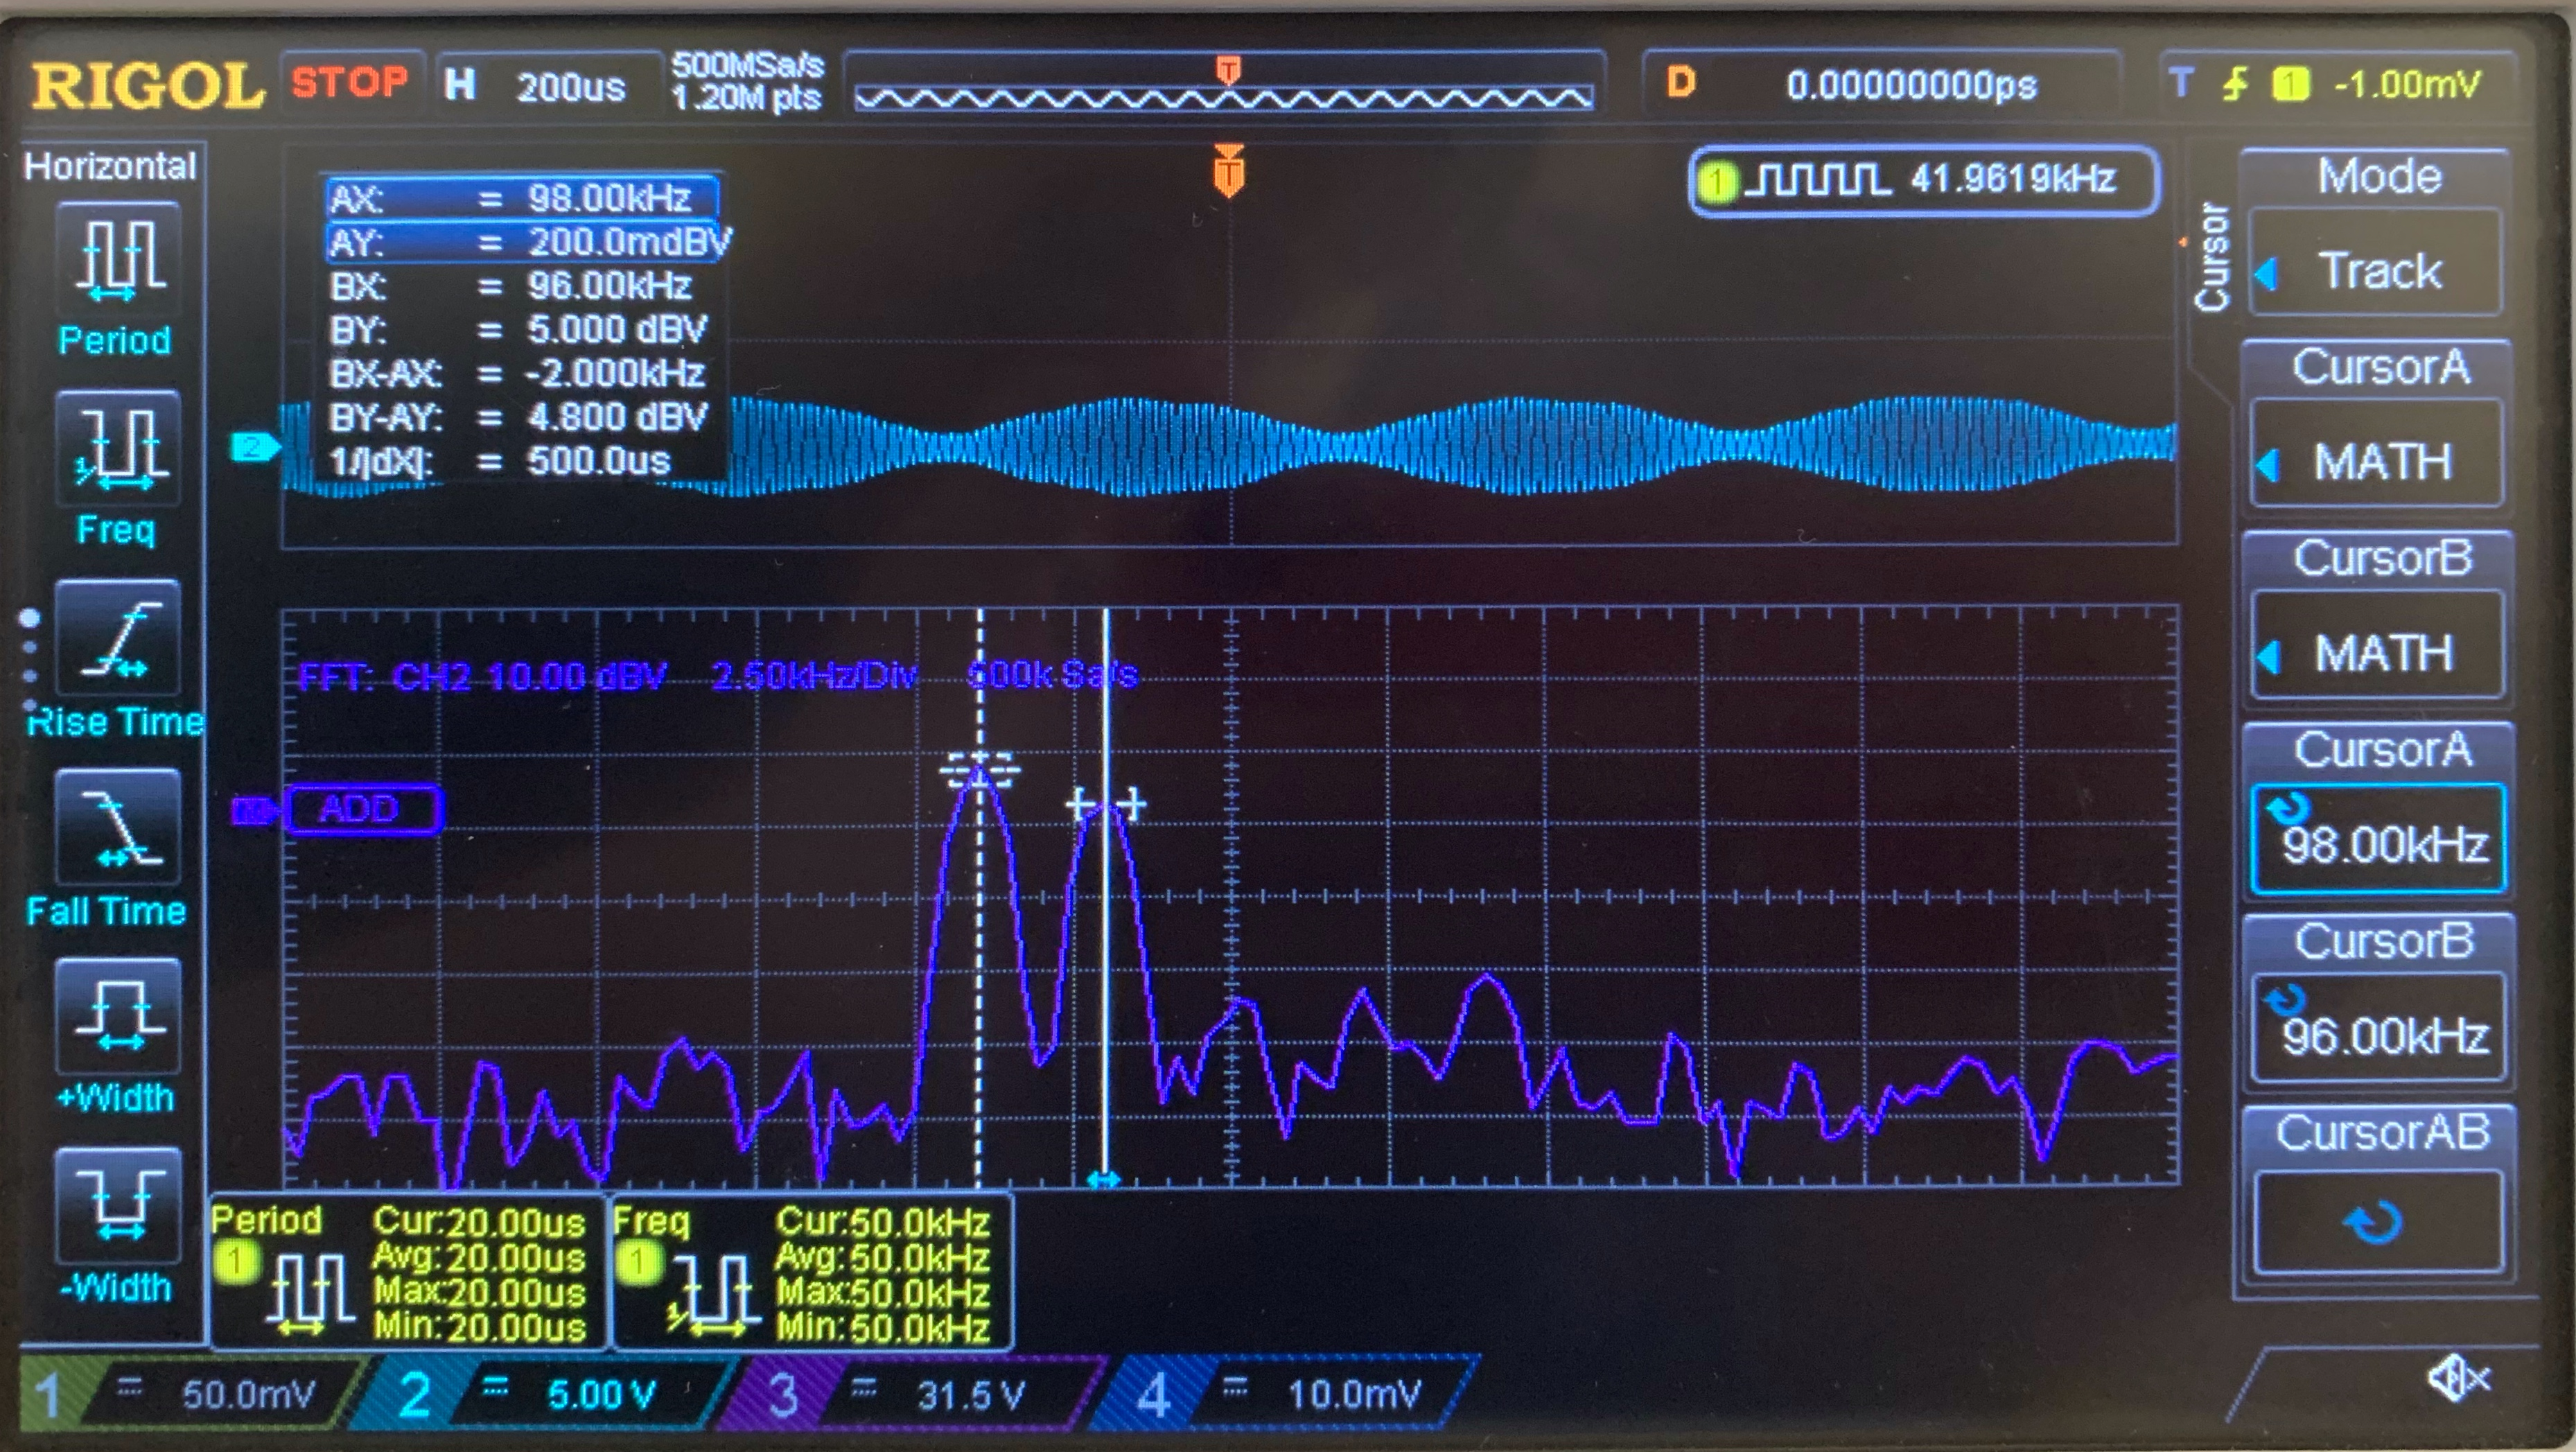
\includegraphics[width=15cm]{W3Q1bc.jpg}
    \caption{Time and frequency domain representations of the SSB signal}
    \label{fig:W3Q1bc}
\end{figure}
\end{enumerate}

\subsection*{Configuration Sketch}
\begin{figure}[H]
    \centering
    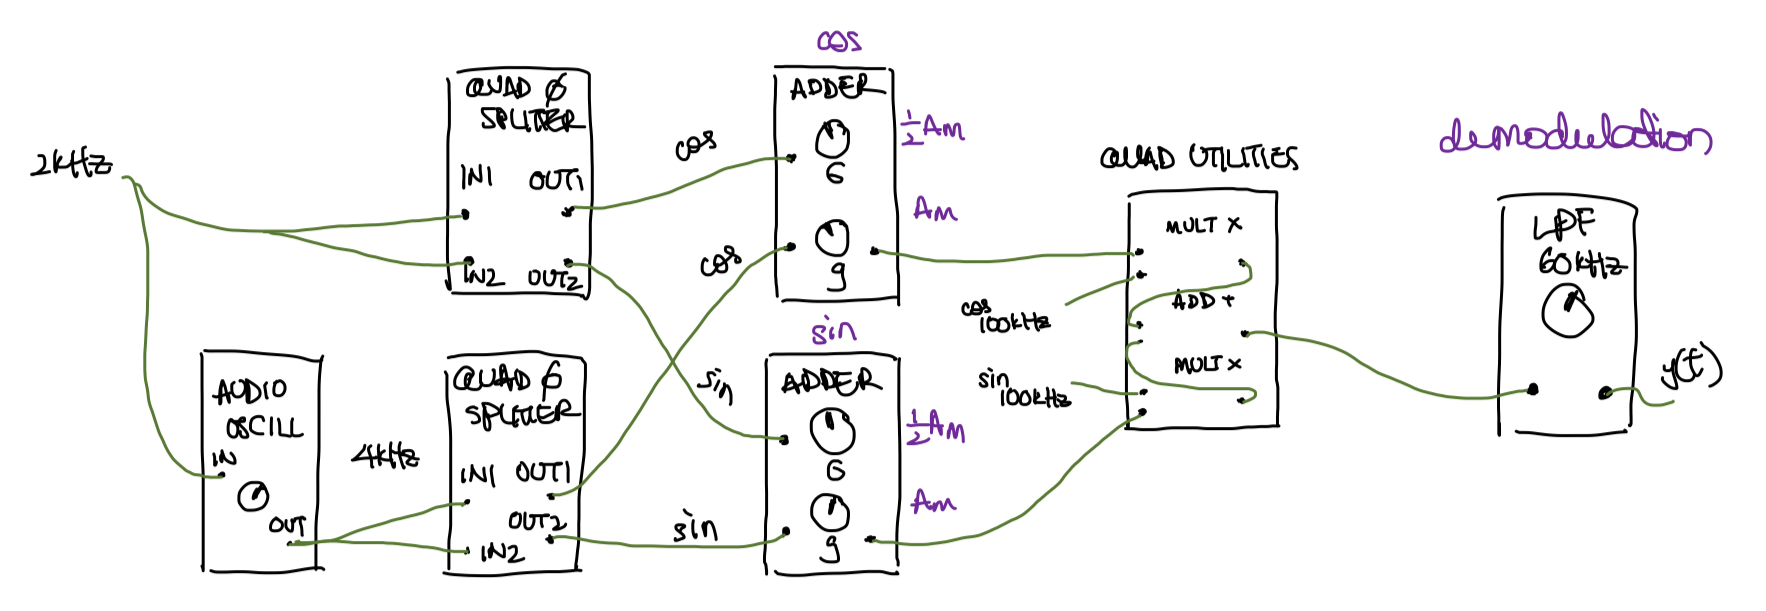
\includegraphics[width=14cm]{W3Q1_2Config.jpeg}
    \caption{Configuration sketch of generating and modulating the SSB signal as well as following through to the LPF for Q2}
    \label{fig:W3Q1_2Config}
\end{figure}
%% good sketching

\newpage
\section*{Question 2}
\begin{enumerate}[label=(\alph*)]
\item SSB signal can be demodulated by multiplying with a stolen carrier $\tilde{v}_c(t)=cos(2\pi f_c t)$ and passing through a low pass filter. Recall what we had for $s(t)$ in time-domain:
\begin{align*}
    s(t)=\frac{A_c}{2} \biggr (m(t)\cos(2\pi f_c t) \pm \tilde{m}(t)\sin(2\pi f_c t) \biggr)
\end{align*}
The mixed signal can be expressed as:
\begin{align*}
    s(t)\tilde{v}_c(t)=\frac{A_c}{2} \biggr (m(t)\cos(2\pi f_c t)\cos(2\pi f_c t) \pm \tilde{m}(t) \sin(2\pi f_c t) \cos(2\pi f_c t) \biggr)
\end{align*}
where,
\begin{align*}
    m(t)=\frac{1}{2} \cos(2\pi f_m t)+ \cos(2\pi 2f_m t) \\
    \tilde{m(t)}=\frac{1}{2}\sin(2\pi f_m t)+ \sin(2\pi 2f_m t)
\end{align*}
We now re-write $\tilde{v}_c(t)$ as
\begin{align*}
    \tilde{v}_c(t)= \cos(2\pi f_c t)=\frac{e^{j2\pi f_c t }+e^{-j2\pi f_c t }}{2}
\end{align*}
By knowing that $x(t)e^{j2\pi f_c t }$ after Fourier transform will become $X(f-f_c)$, it discloses a quick way to write down the frequency domain expression of $s(t)\tilde{v}_c(t)$ using $S(f)$: \\
(Because we are taking real world experiments to see the spectrum, only either $+$ or $-$ sign will be choose. We suppose $+$ is picked to see the lower sideband mixing components.)
\begin{align*}
    \mathcal{F}\{s_{+}(t)\tilde{v}_c(t)\}= \frac{A_c}{16}\bigg ( \delta(f-(2f_c-f_m))+\delta(f-f_m)+\delta(f+f_m)+\delta(f-(f_m-2f_c)) \\
    +2\delta(f-(2f_c-2f_m))+2\delta(f-2f_m)+2\delta(f+2f_m)+2\delta(f-(2f_m-2f_c)) \bigg )
\end{align*}
whereas upper sideband mixing components can be found by picking $-$ sign:
\begin{align*}
    \mathcal{F}\{s_{-}(t)\tilde{v}_c(t)\}= \frac{A_c}{16}\bigg ( \delta(f-(2f_c+f_m))+\delta(f+f_m)+\delta(f-f_m)+\delta(f+(f_m+2f_c)) \\
    +2\delta(f-(2f_c+2f_m))+2\delta(f+2f_m)+2\delta(f-2f_m)+2\delta(f-(2f_m+2f_c)) \bigg )
\end{align*}
For both case, we expect 8 spikes over the whole spectrum with 4 in the positive frequencies.

We forgot to take a picture of this one, but this has been checked by our demonstrator (see sign offs).

\item %b 
As we want to keep the terms of frequencies on $\pm f_m$ and $\pm 2f_m$, we need the lowpass filter to filter out all the frequency components above $\pm 2f_m (4kHz)$. The lowest needless frequency is on $2f_c - 2f_m$ which is $196kHz$. We can choose any filter with 3-dB bandwidth between $4k Hz$ and $196k Hz$. 
\item %c
We sent the mixed signal to a 60kHz Lowpass filter, the output signal from LPF is the demodulated one. The demodulated signal is in yellow shown in Figure \ref{fig:W3Q2c}. The blue signal is the original time domain message. The only two remaining spikes were located in 2kHz and 4kHz respectively, which indicated a successful demodulation. Noise components in spectrum was reduced after adjusting the offset (not shown in the graph). 
\begin{figure}[H]
    \centering
    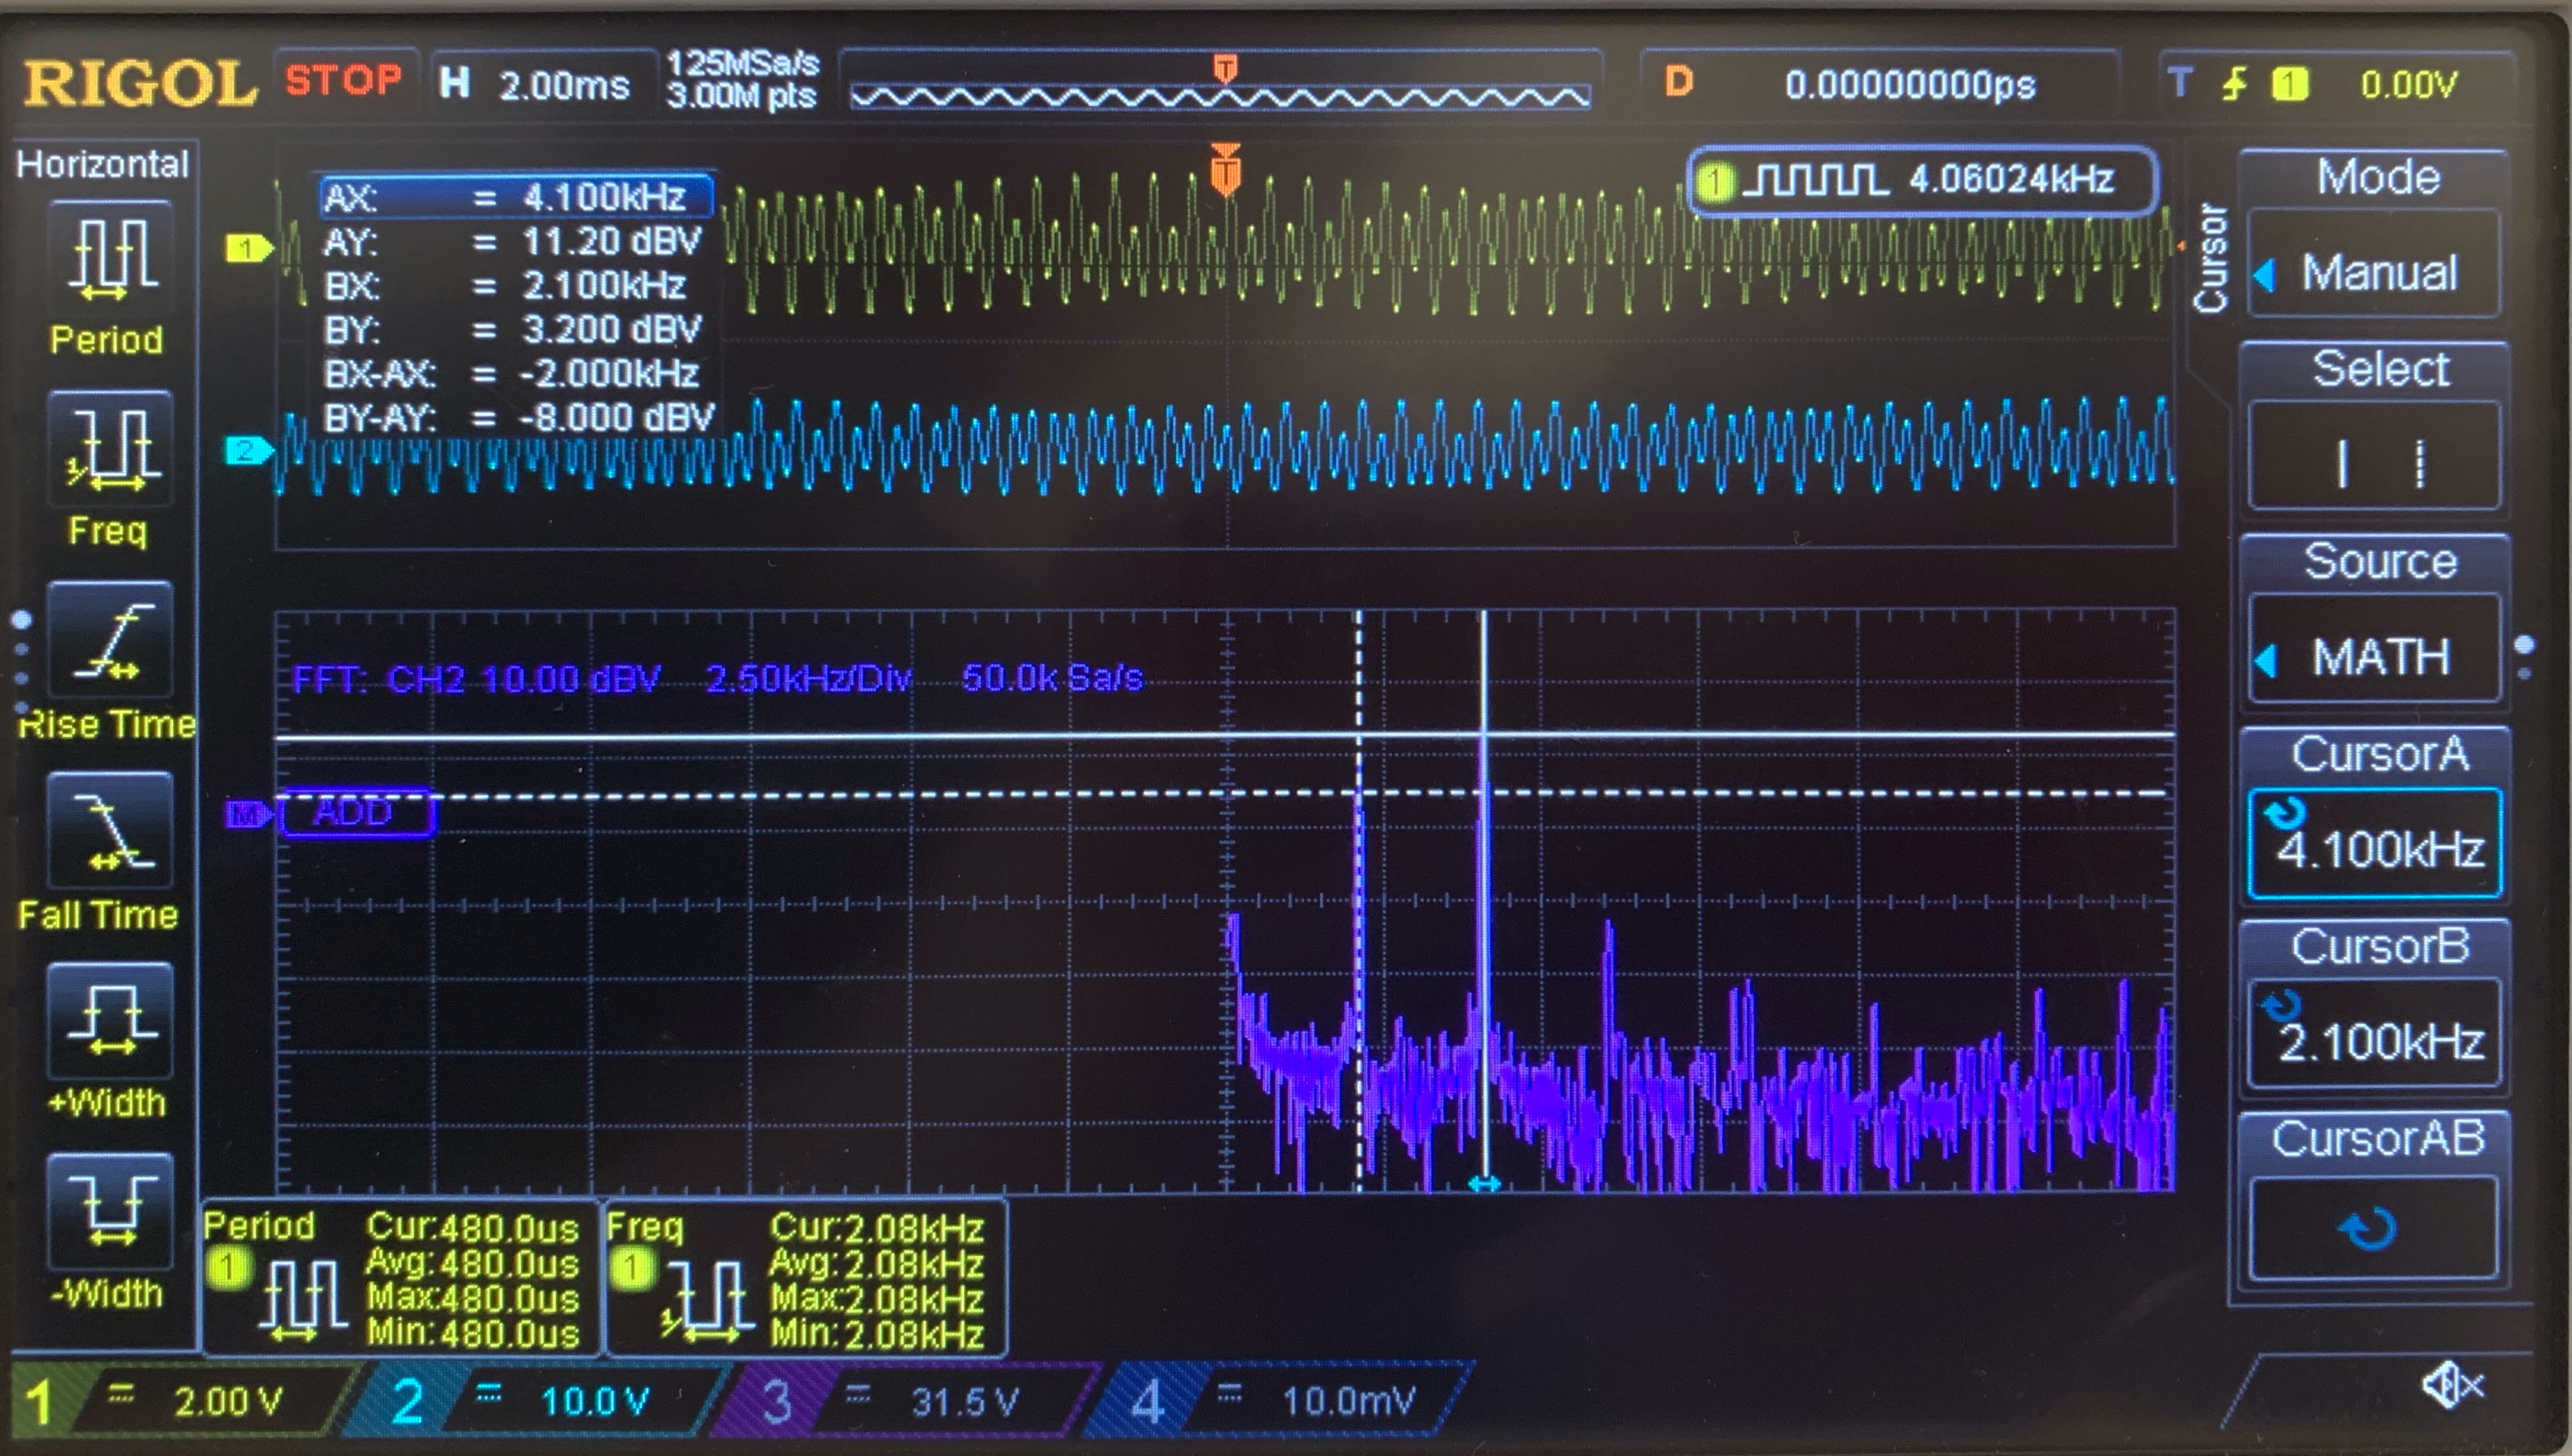
\includegraphics[width=15cm]{W3Q2c.jpg}
    \caption{Time and frequency domain representations of the demodulated SSB signal}
    \label{fig:W3Q2c}
\end{figure}
\textit{Note that the amplitude shows gain after demodulation due to the doubling factor from the phase shift added terms after carrier modulation.}
\end{enumerate}
\section*{Question 3}
\begin{enumerate}[label=(\alph*)]
\item With the absence of any input voltage, we measured the output frequency of the voltage controlled oscillator (VCO) in high frequency mode and low frequency mode respectively. The output frequencies were roughly as expected, and they have been checked by our demonstrators.  
\item Figure \ref{fig:vco} shows the recorded frequencies from high frequency mode and low frequency mode of VCO when we varied the magnitude of input DC voltage. Generally, frequency is positively proportional to input voltage. In both LO and HI mode, our measurements were found within the linear region. The slopes which are the frequency sensitivity $k_f$ were calculated as 13.2 and 2.8 for HI and LO respectively.
\begin{figure}[H]
    \centering
    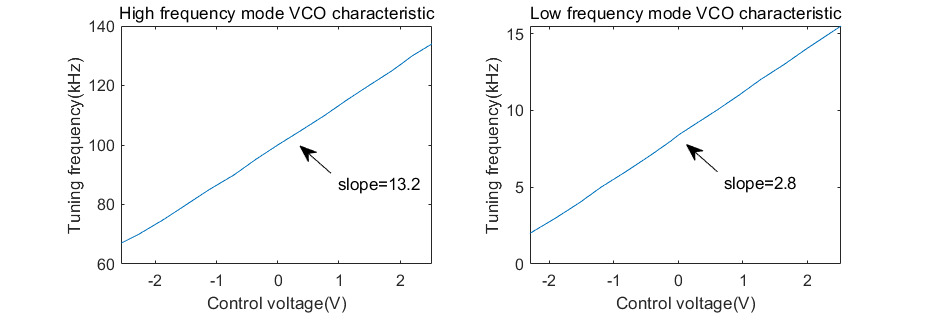
\includegraphics[scale=0.7]{VCOplot.png}
    \caption{VCO characteristic in high frequency mode and low frequency mode.}
    \label{fig:vco}
\end{figure}

Using the second method, we sent a pure sinusoid signal with frequency $W=2$kHz ($m(t)=A_m \cos{2\pi Wt}$) to the HI VCO. Initially, we set $A_m$ to be a small value, we observe the FFT of the VCO output signal mainly at the center frequency. With increasing $A_m$, the spike at center frequency gradually decreasing until zero. At this moment, $A_m$ was measured as approximately 0.4V, which leads to a calculation on $k_f$ by $\beta=\frac{k_f A_m}{W}$. Knowing that $\beta=2.4$ when the center frequency spike reached zero, therefore $k_f$ is calculated as 12. This is roughly in agreement with our VCO HI characteristic above. Note that the magnitude of other spikes changed along with varying $A_m$ as well. But only the first two spikes are significant.  

\item % c
As shown in Figure \ref{fig:Q3cplot}, the expected spectrum of $\beta=2$ was sketched by checking the Bessel chart from textbook. The relative data were obtained as: $J_0(2)=0.22,J_1(2)=0.58,J_2(2)=0.35,J_3(2)=0.13,J_4(2)=0.03, J_5(2)=0.01$. The negative side is subject to a mirror image of the positive side. Between each of the two spikes, the distance is corresponding to the frequency of the message signal $W$. 
\begin{figure}[H]
    \centering
    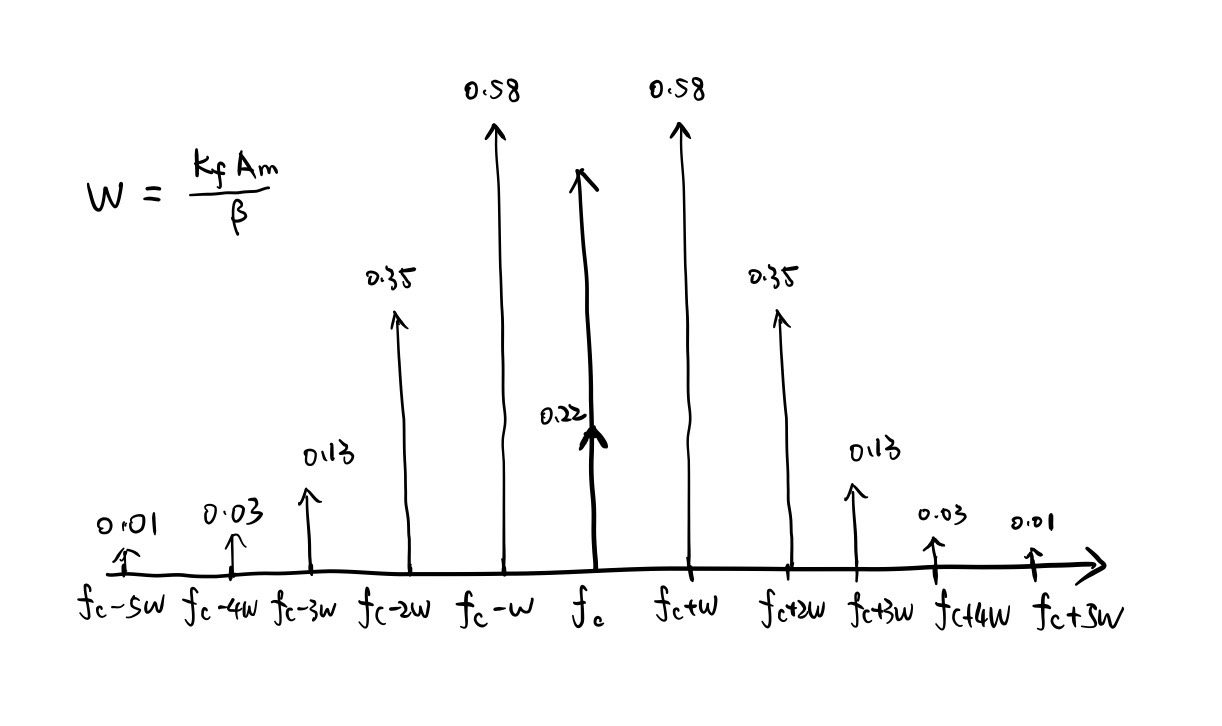
\includegraphics[scale=0.25]{W3Q3c.jpg}
    \caption{Expected spectrum when $\beta=2$.}
    \label{fig:Q3cplot}
\end{figure}
% What's the extra peak at f_c is this DC?

% that is J_0. f_c = 100kHz, so its not DC.

\item %d
We computed $k_f$ using the Bessel zero method in sub-question b). There were small discrepancies between the VCO characteristic and the Bessel zero approach. The VCO characteristic method is considered more precise as it adopted detailed data, and taking slope of it has neglect some errors in the data points. However, in the second approach, center frequency spike is observed by the human eye which led to errors. And the FFT mode of scope has some noise components as well. 
\end{enumerate}

\subsection*{Configuration Sketch}
\begin{figure}[H]
    \centering
    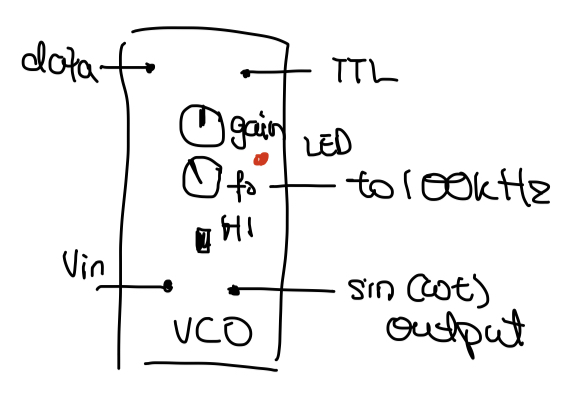
\includegraphics[width=5cm]{W3Q3Config.jpeg}
    \caption{Configuration sketch of the VCO module}
    \label{fig:W3Q3Config}
\end{figure}

\newpage
\section*{Question 4}
\begin{enumerate}[label=(\alph*)]
\item %a
Our FM signal output is shown in Figure \ref{fig:W3Q4a}. It can be seen that the waveform is unevenly distributed due to a varying frequency in the signal, which is signature to a FM modulated signal. 
\begin{figure}[H]
    \centering
    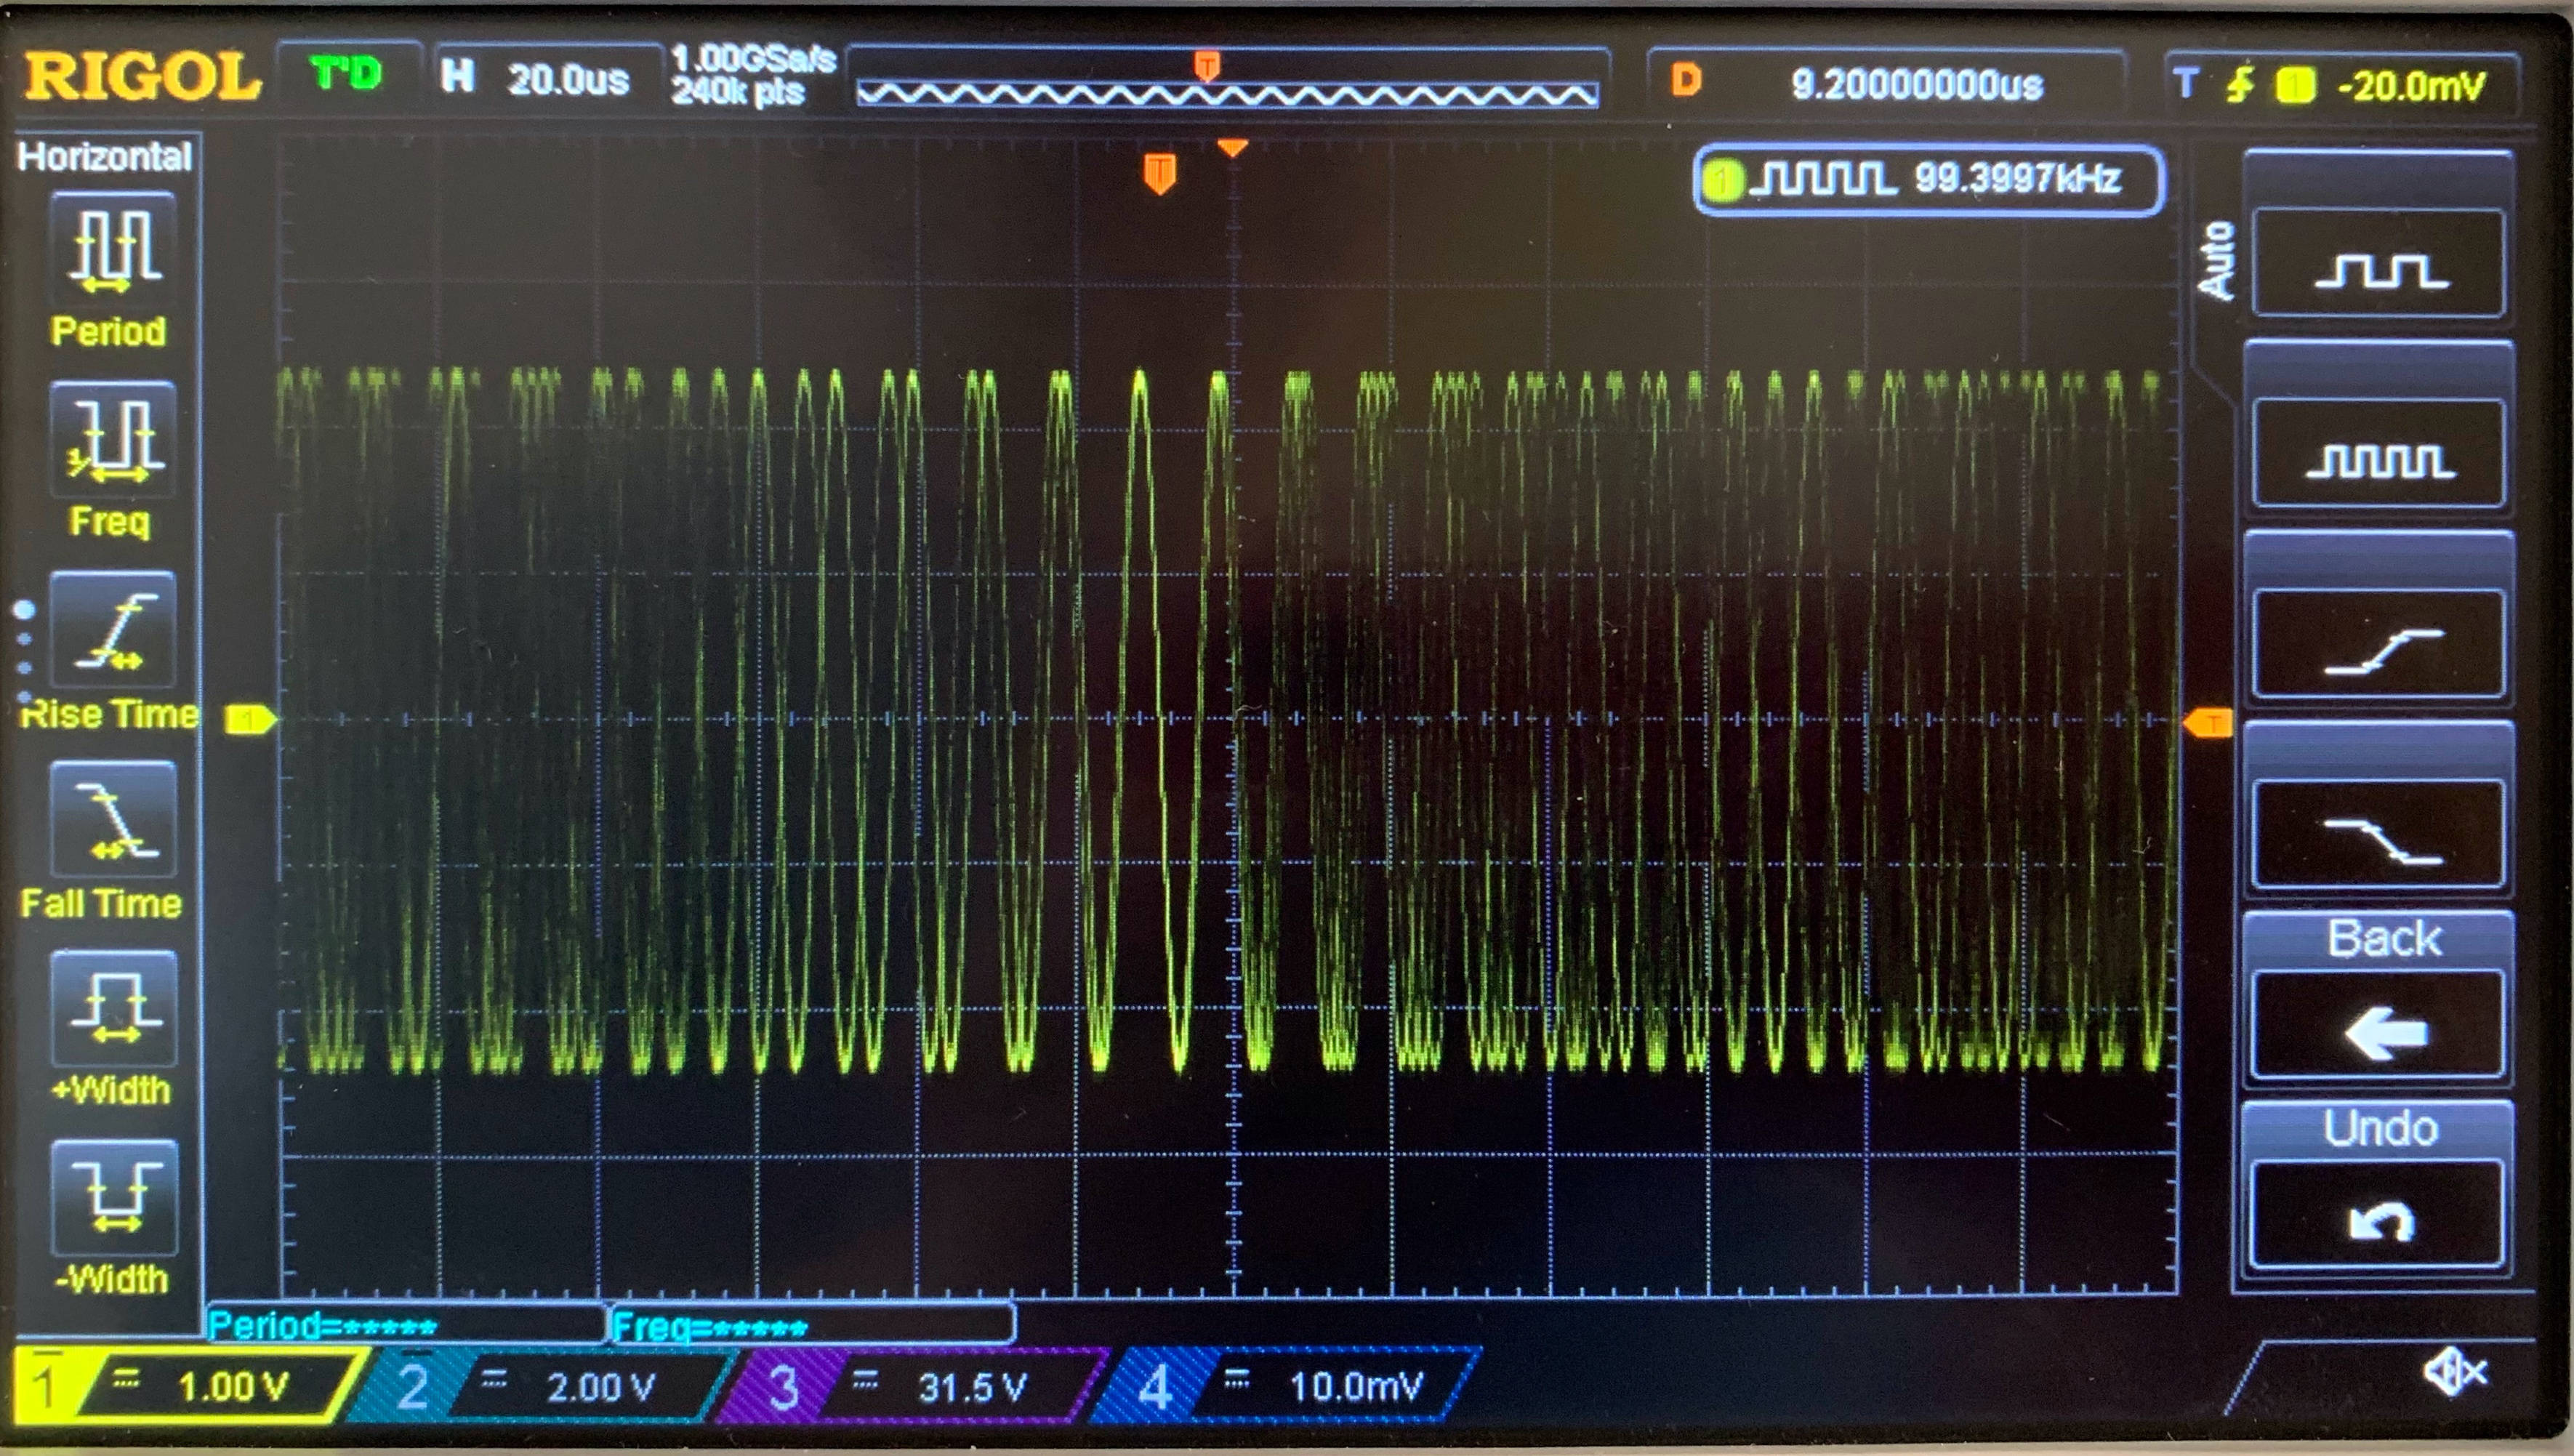
\includegraphics[width=15cm]{W3Q4a.jpg}
    \caption{FM signal generated via a VCO}
    \label{fig:W3Q4a}
\end{figure}
\item %b
For this part we adjusted the VCO module gain to generate different $\beta$ values. 

\begin{enumerate}
    \item %i beta = 1.4 Am=0.22
    At $\beta = 1.4$, we expect the centre and immediate side peak to be of the same magnitude according to Bessel chart. This is coherent with our observations in the FFT in Figure \ref{fig:W3Q4bB1_4}. With our experimental $k_f$ of 13.2, we expected $A_m$ to be 0.212V with $W=2kHz$ and this is very close to our measured $A_m$ of 0.22V. 
    The Carson's bandwidth for $\beta = 1.4$ is $B = 2(1 + \beta)W = 9.6$kHz. However, the bandwidth required from our spectrum is around 14kHz. Carson's rule had underestimated the bandwidth for $\beta=1.4$. 
    \begin{figure}[H]
    \centering
    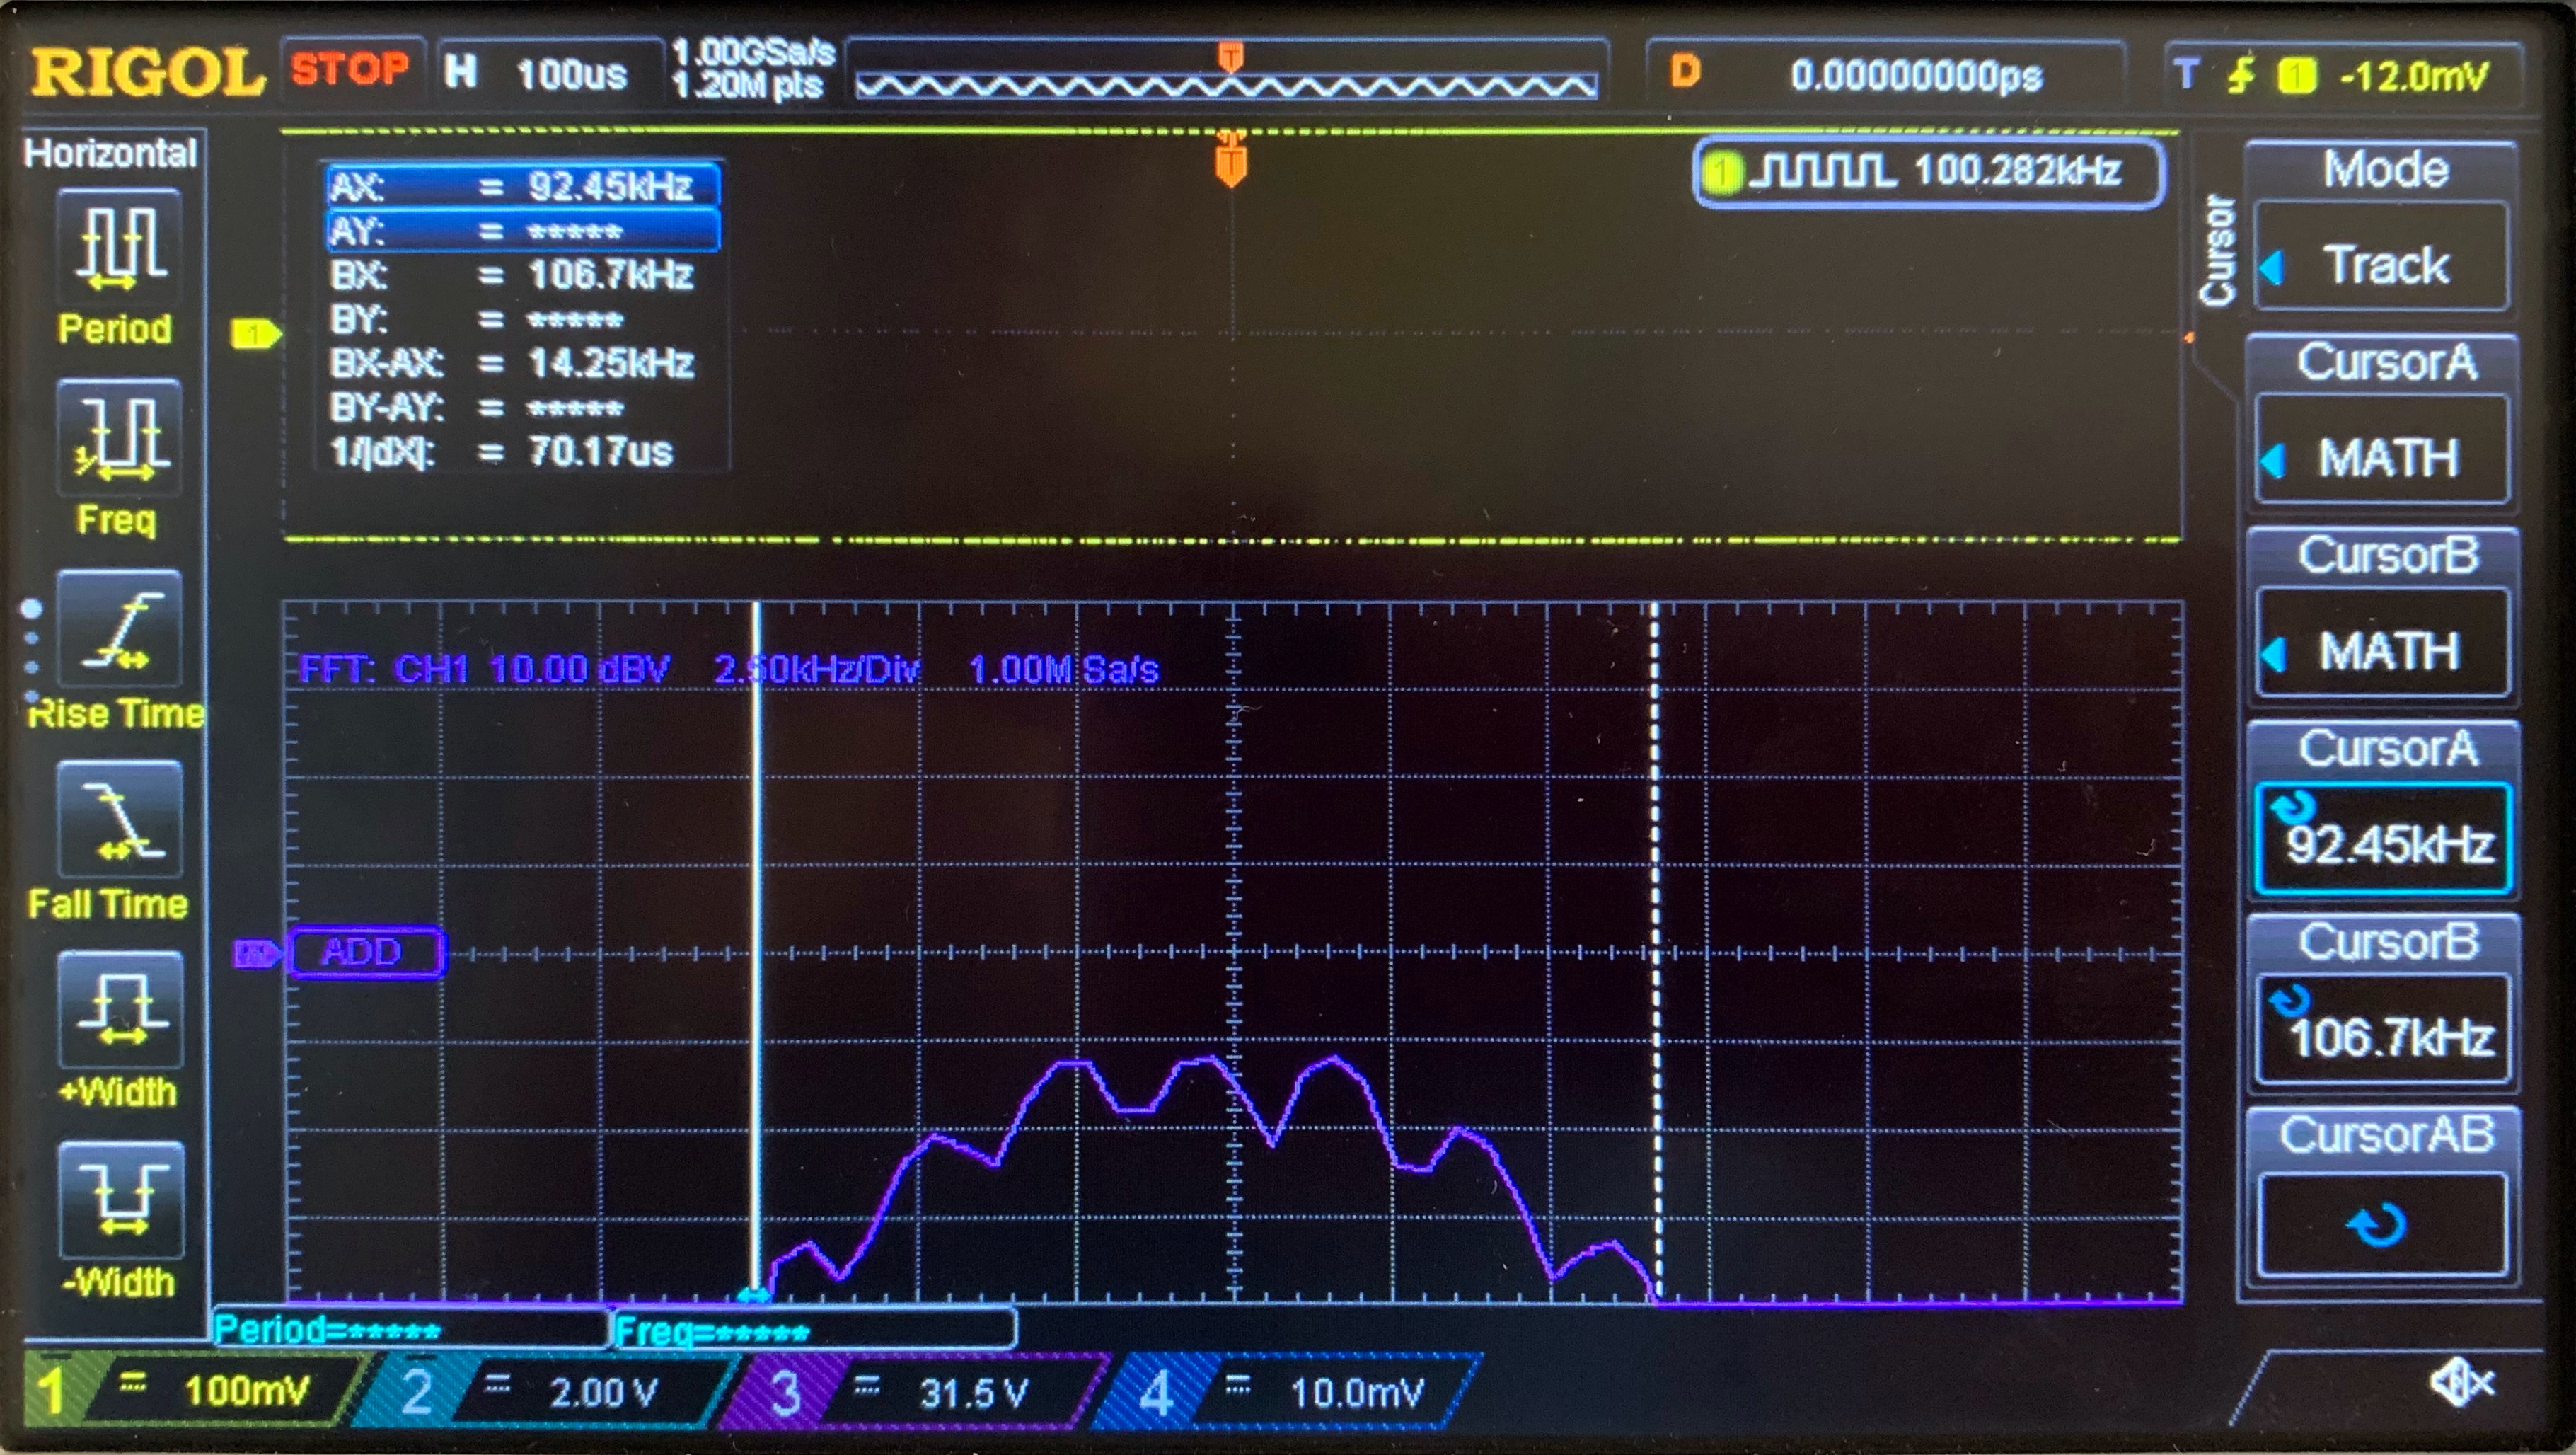
\includegraphics[width=15cm]{W3Q4bB1_4.jpg}
    \caption{FM modulated signal of $\beta$ = 1.4}
    \label{fig:W3Q4bB1_4}
    \end{figure}
    
    \item %i beta = 2 Am=0.3
    As per our drawing sketch in Q3 c), we expect the centre peak to be lower than the immediate ($J_1$) and second immediate ($J_2$) peaks. The tallest peaks that are present should be the immediate side lobe $J_1$ as seen in our FFT in Figure \ref{fig:W3Q4bB2}. Using our experimental $k_f$ again, we calculate $A_m$ as 0.303V, which is our measured $A_m$ of 0.3 with $W=2kHz$. There seems to be a fair bit of noise as well, which may have swamped the additional side peaks. 
    The Carson's bandwidth for $\beta = 2$ is $B = 2(1 + \beta)W = 12$kHz, which is way underestimating the bandwidth for $\beta=2$. 
    \begin{figure}[H]
    \centering
    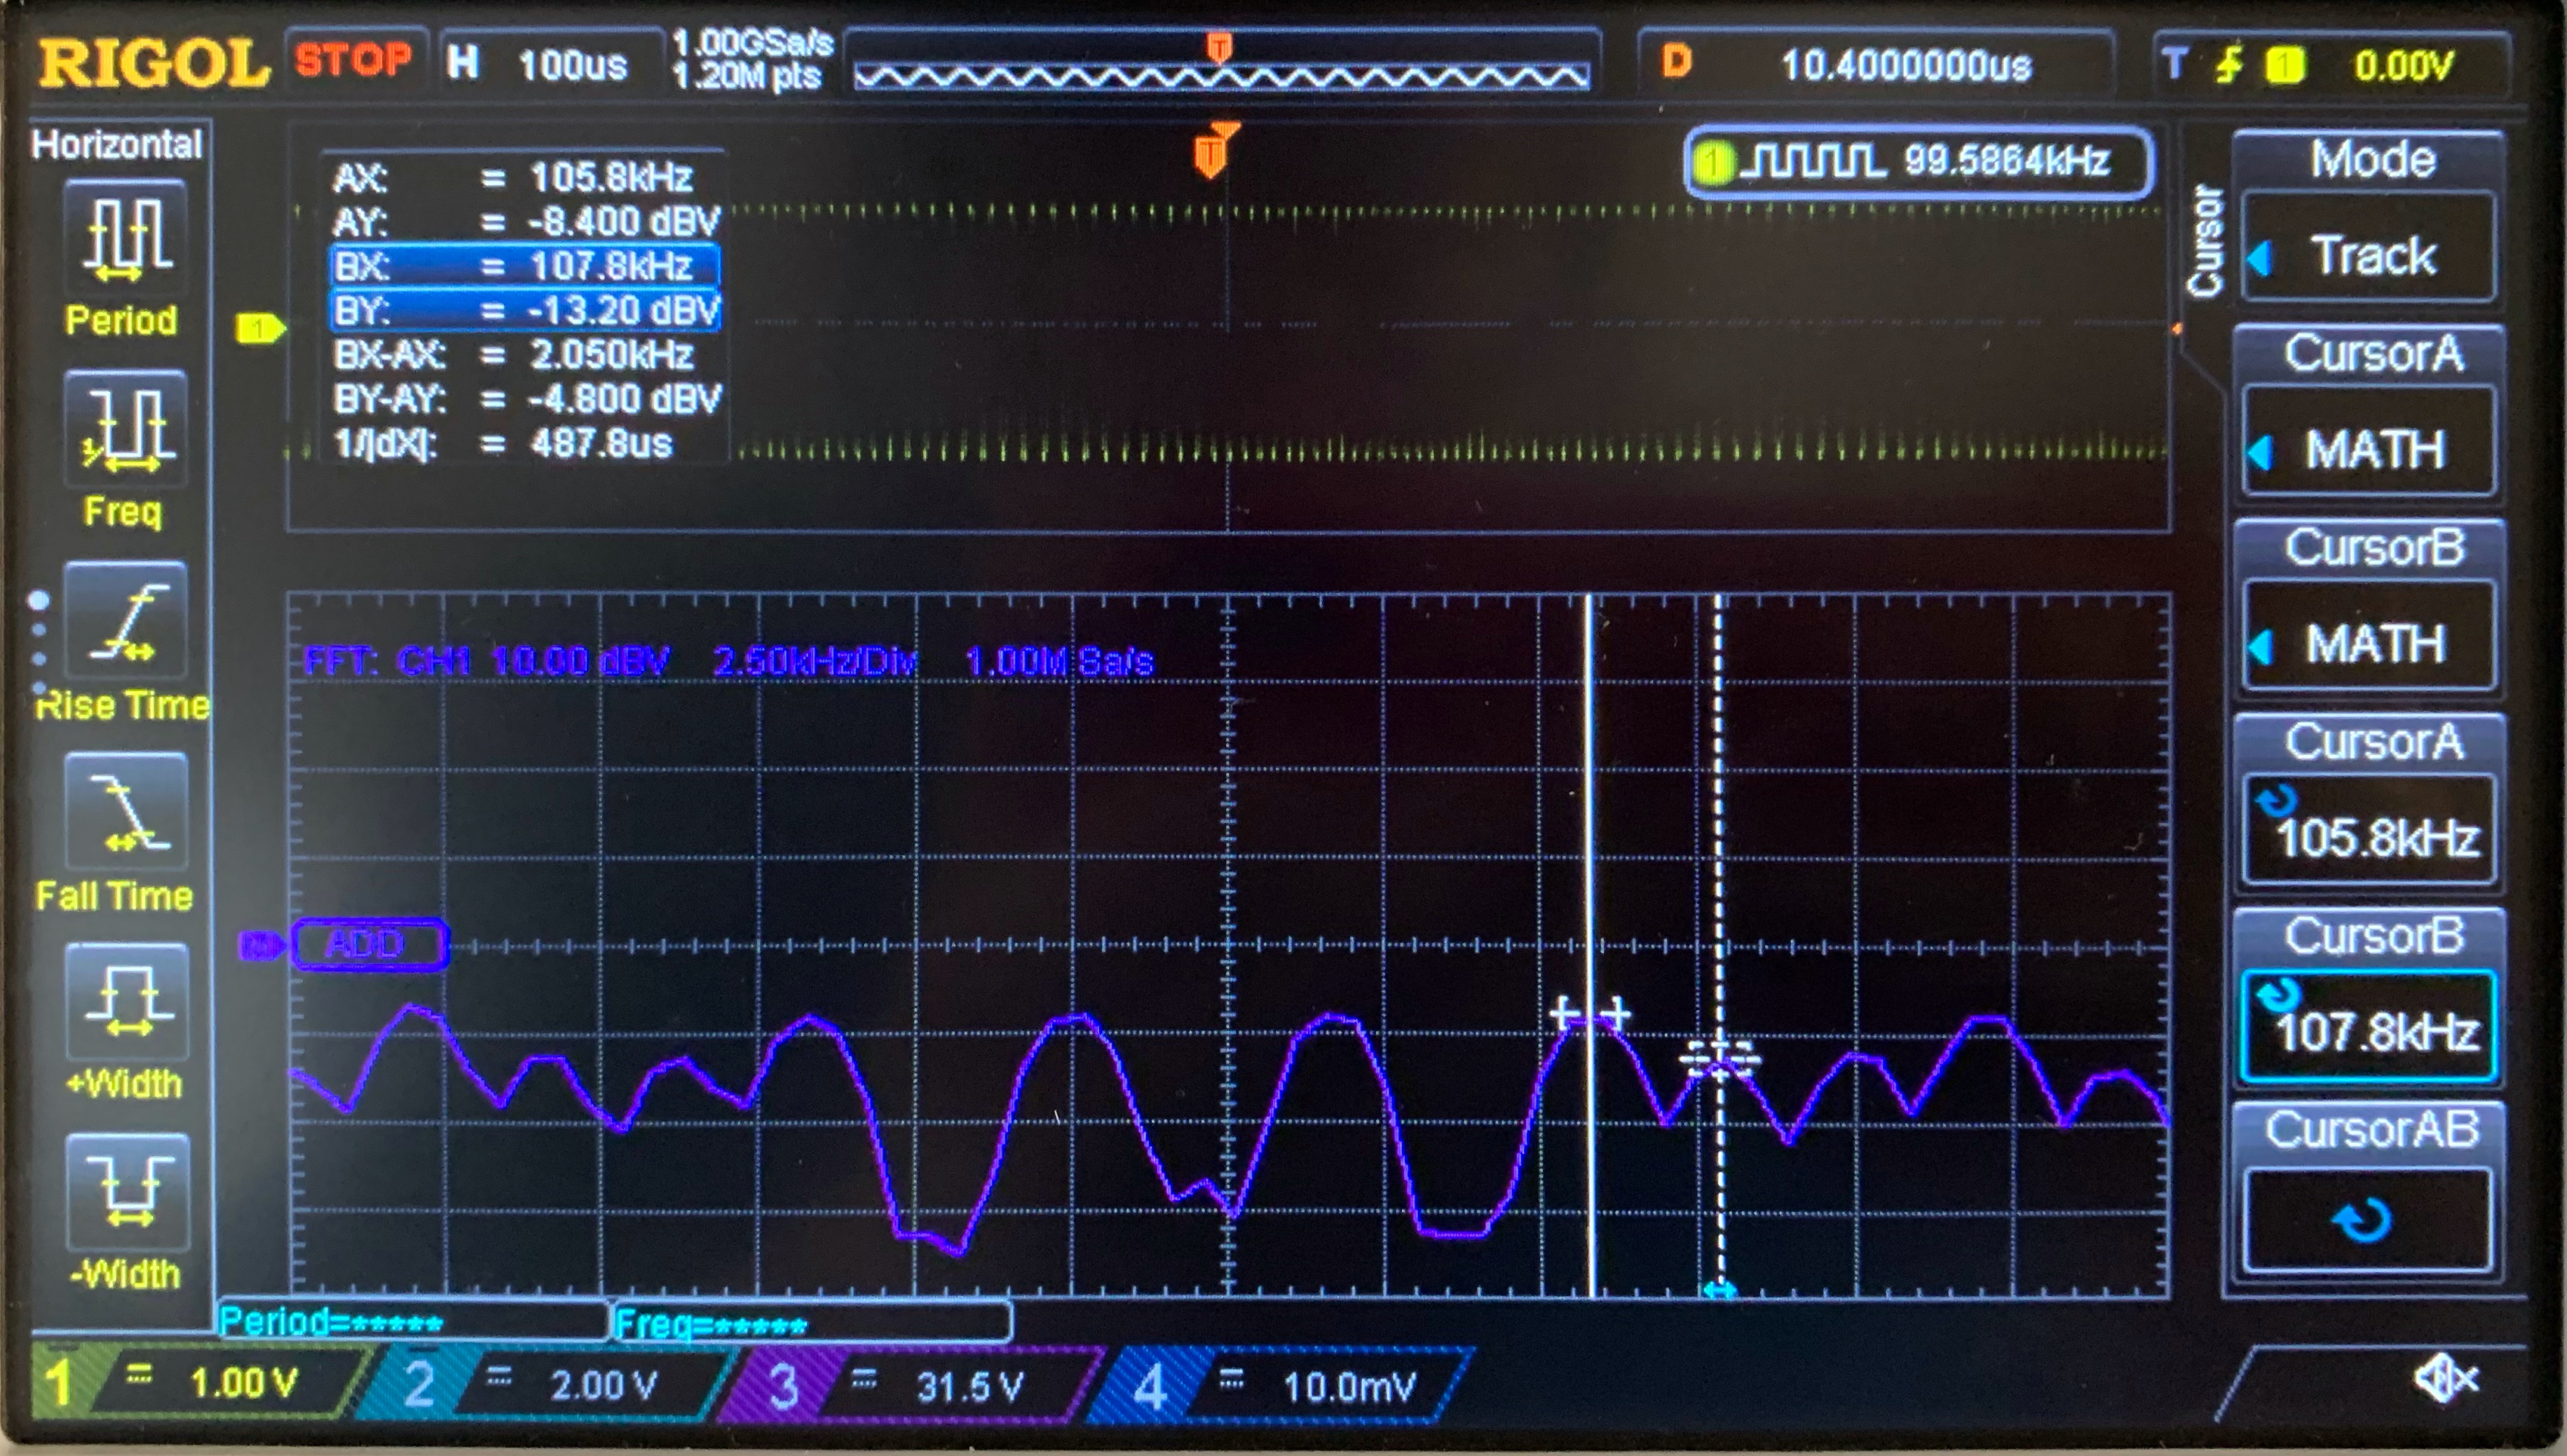
\includegraphics[width=15cm]{W3Q4bB2.jpg}
    \caption{FM modulated signal of $\beta$ = 2}
    \label{fig:W3Q4bB2}
    \end{figure}
    
    \item
    % Am=0.5 beta=3.3
    Again, calculating the $A_m$ using $k_f$ = 13.2 we have 0.5V which is our measured $A_m$. $W$ is still remained to be 2kHz. In Figure \ref{fig:W3Q4bB2_4} we see that the second side lobes are the tallest which is expected from the Bessel function curves. 
    The Carson's bandwidth for $\beta = 3.3$ is $B = 2(1 + \beta)W = 14.2$kHz. However, the experimental required bandwidth is around $20kHz$. These are expected since Carson's bandwidth rule works when $\beta>>1$ or $\beta<<1$. Our choices of $\beta$ is not in the desired range of Carson's rule.
    \begin{figure}[H]
    \centering
    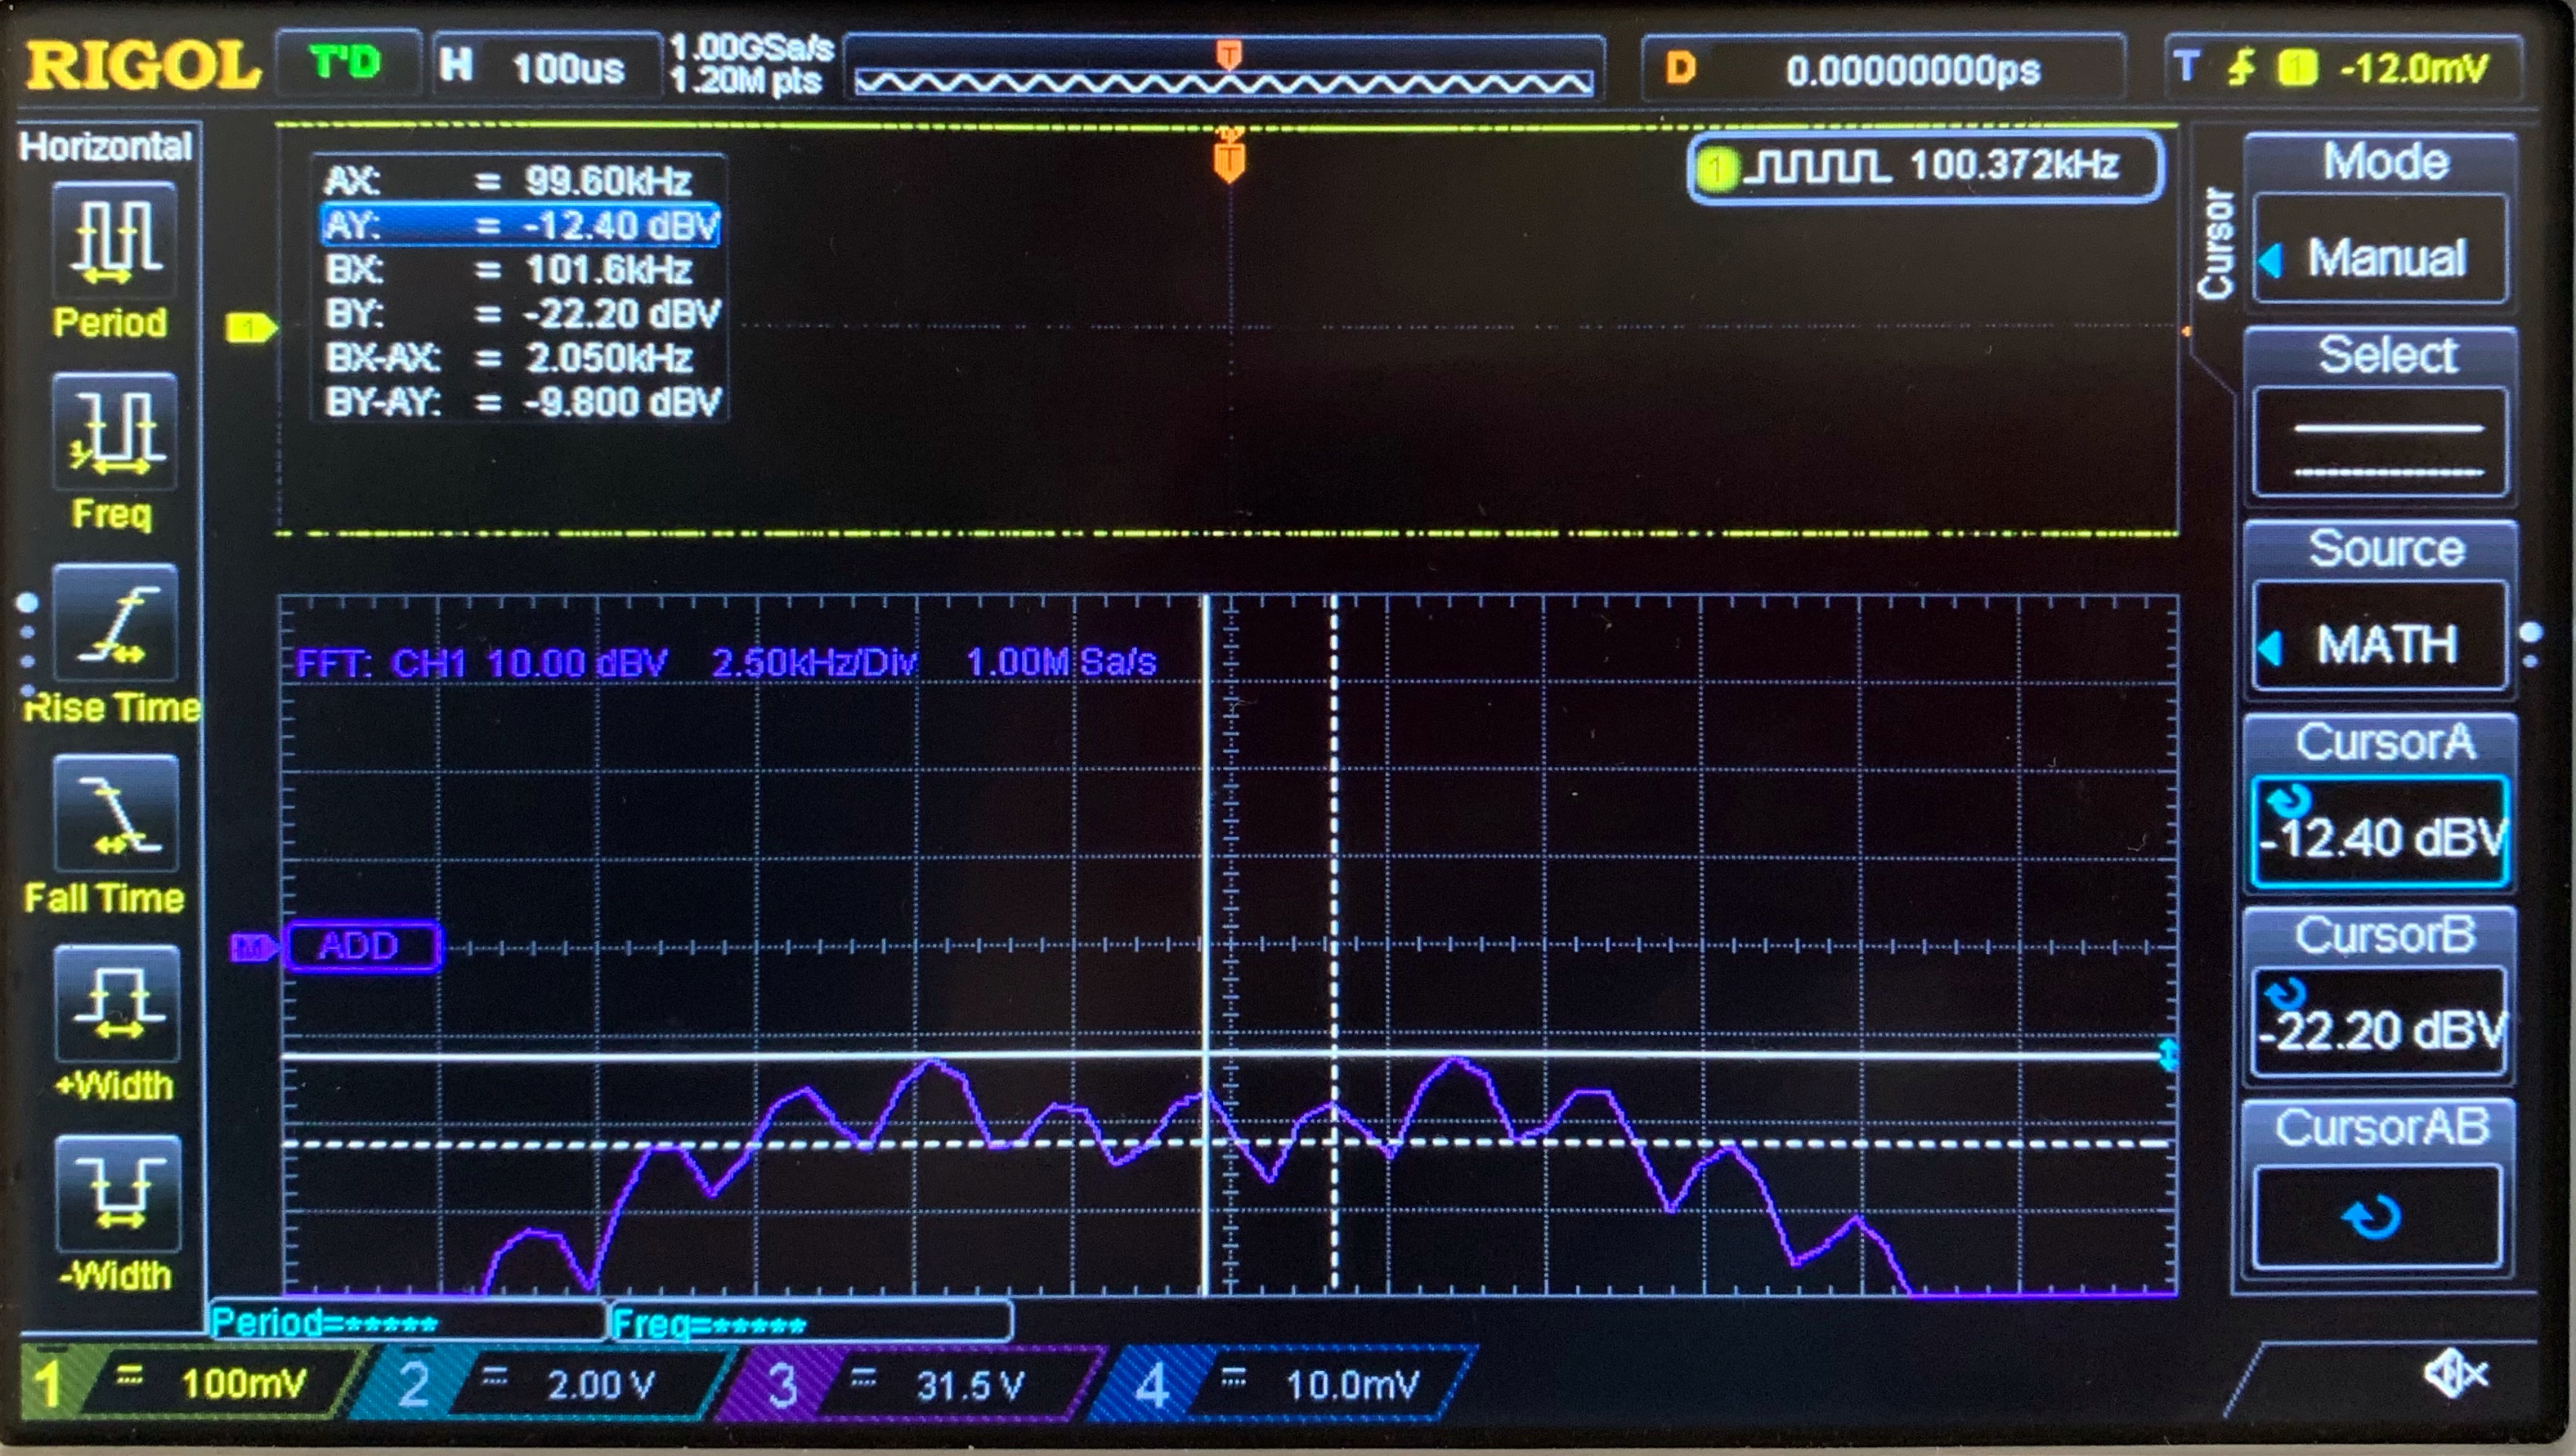
\includegraphics[width=15cm]{W3Q4bB2_4.jpg}
    \caption{FM modulated signal of $\beta$ = 3.3}
    \label{fig:W3Q4bB2_4}
    \end{figure}
\end{enumerate}
Generally, using Bessel chart is an alternative way to roughly determine $\beta$. This method can be used by comparing the relative magnitude between each spikes and refer to Bessel chart for the corresponding $\beta$ value. For instance, when $\beta=1$, the spike in the center ($J_o$) should be close to 0.8, while the first spike has the magnitude around 0.4. Similarly, the second spike will be around 0.1. By adopting this method, an approximate $\beta$ can be determined.
\end{enumerate}

\newpage
\section*{Question 5}
\begin{enumerate}[label=(\alph*)]
\item %a
We tested the zero crossing detector with a 100kHz sine wave which is shown in Figure \ref{fig:W3Q5a}. 
\begin{figure}[H]
    \centering
    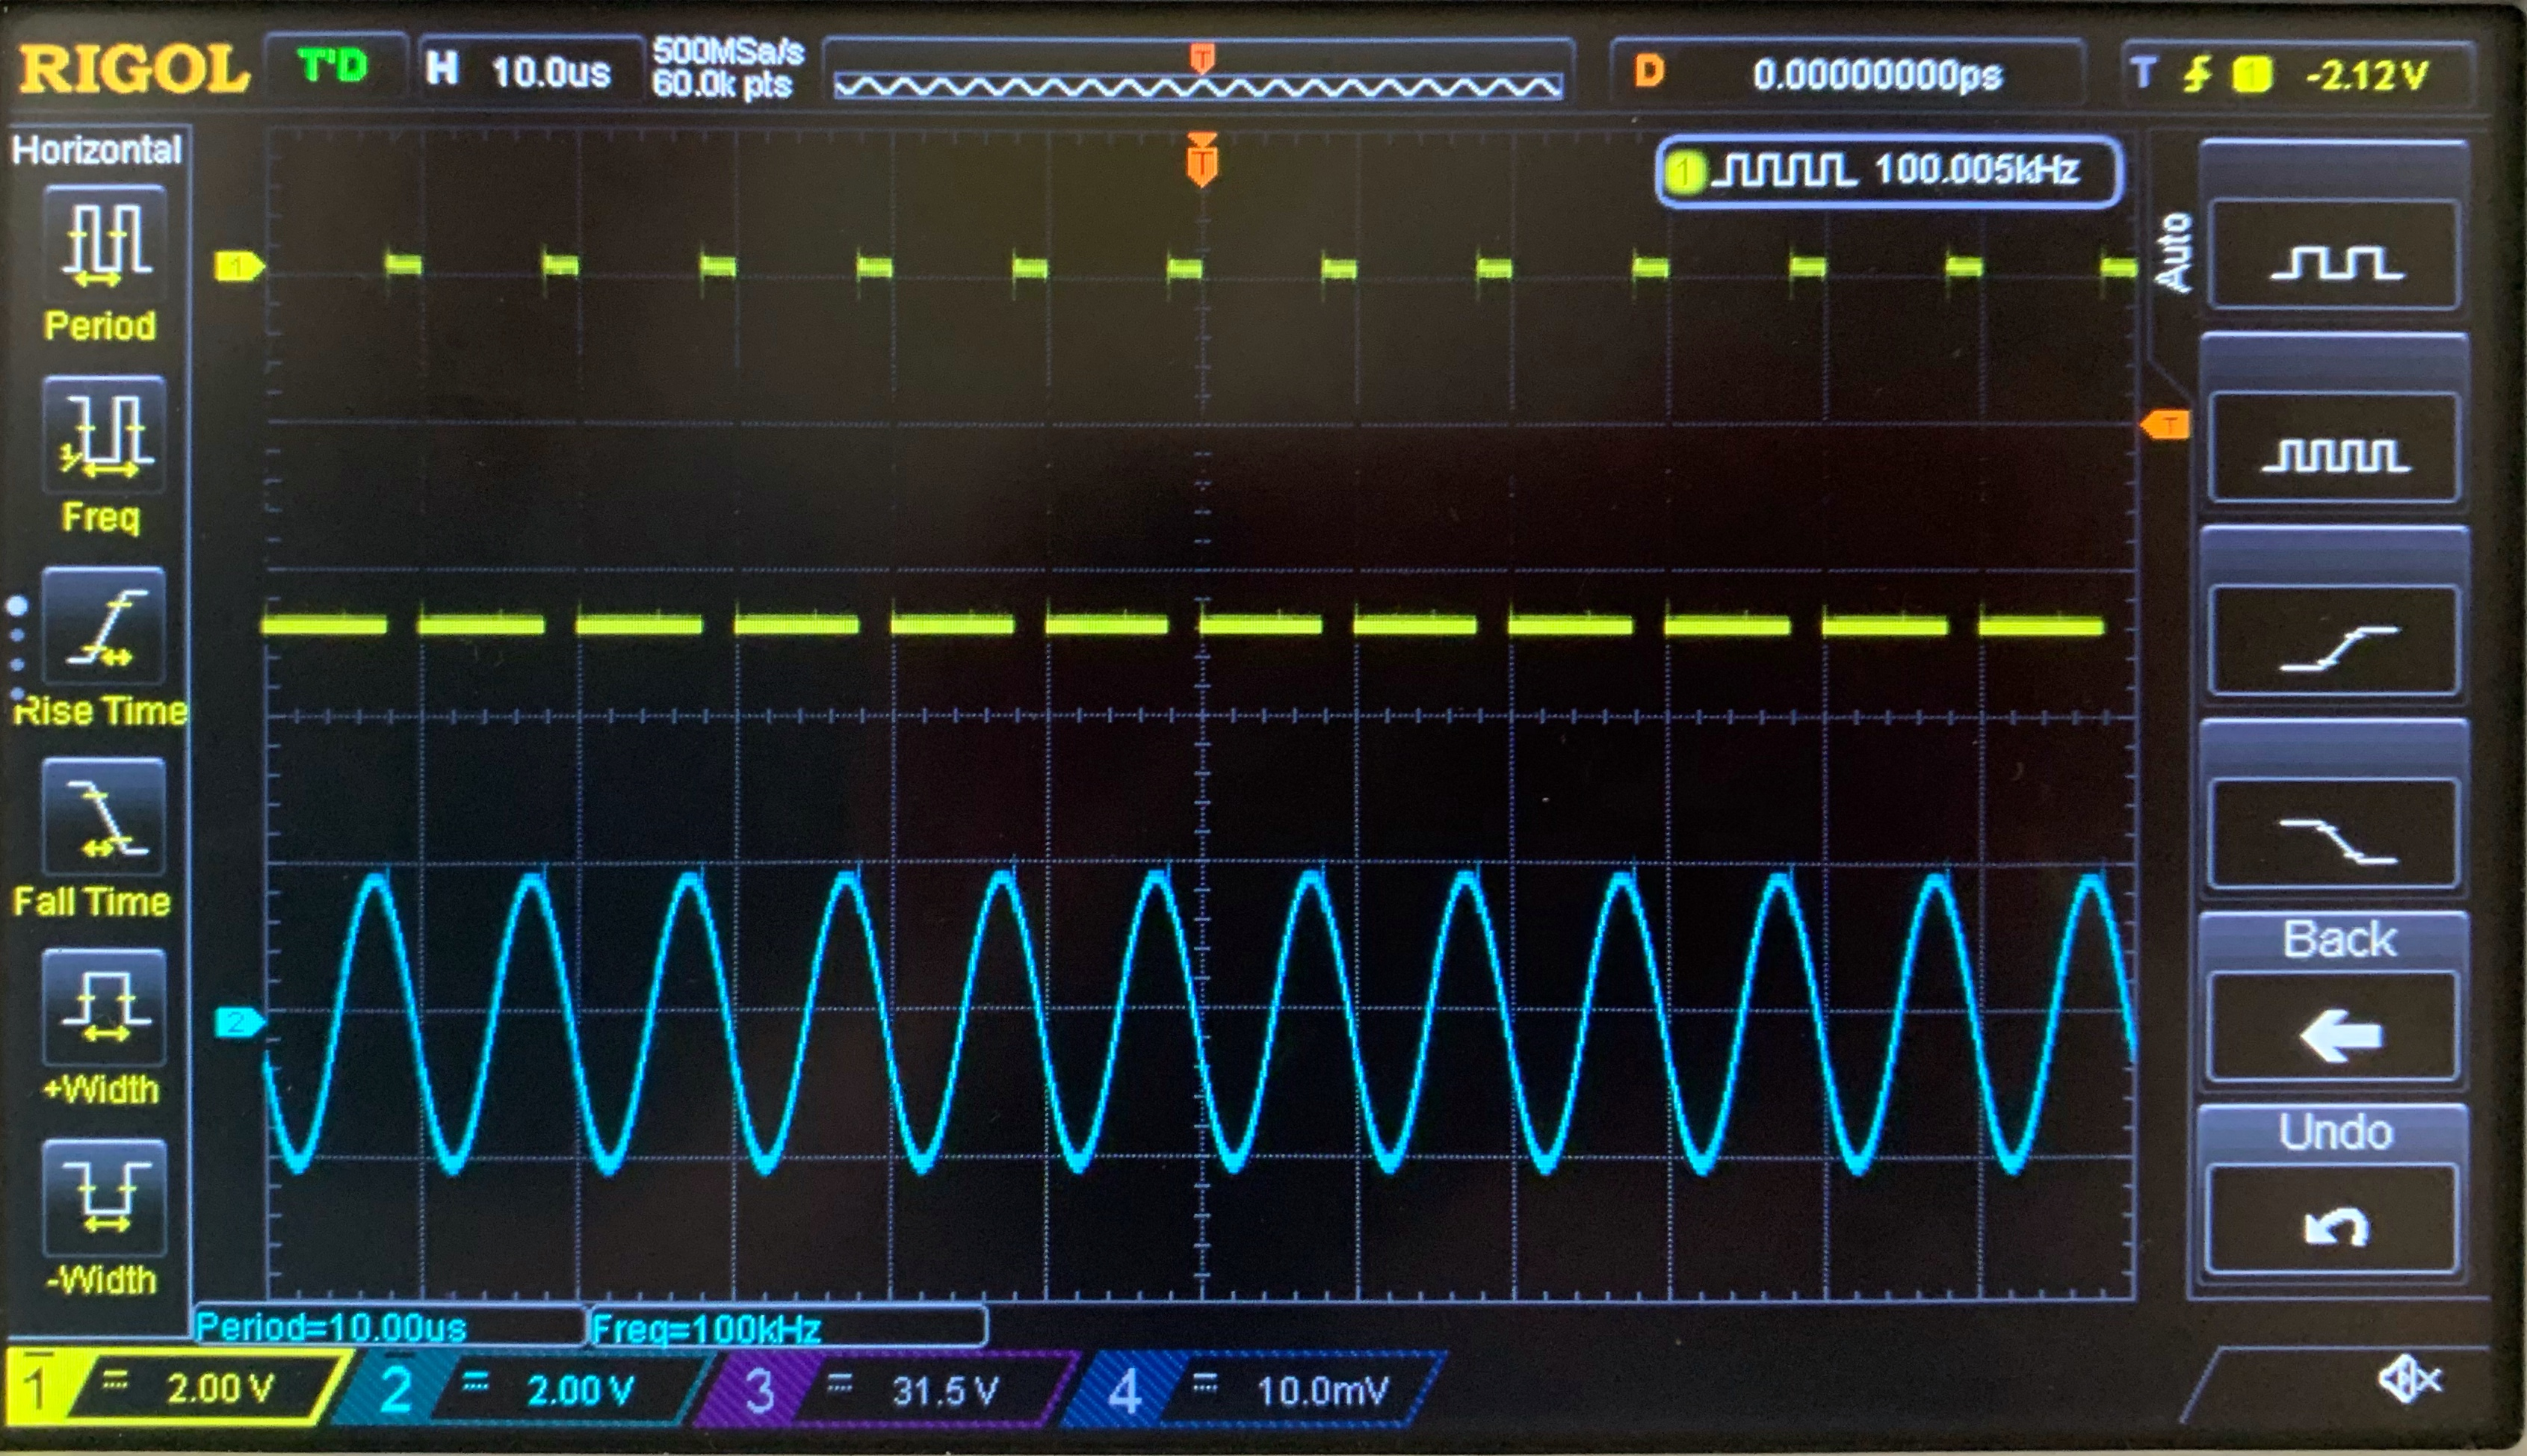
\includegraphics[width=15cm]{W3Q5a.jpg}
    \caption{Zero crossing detection of 100kHz sine wave}
    \label{fig:W3Q5a}
\end{figure}
The optimal choice of pulse width for the non frequency varying signal would be 50\% as this allows the coordination of both rising and falling edges of the zero crossing signal and the square wave input. Figure \ref{fig:W3Q5a_} shows the pulse width of the zero crossing detection output. 
\begin{figure}[H]
    \centering
    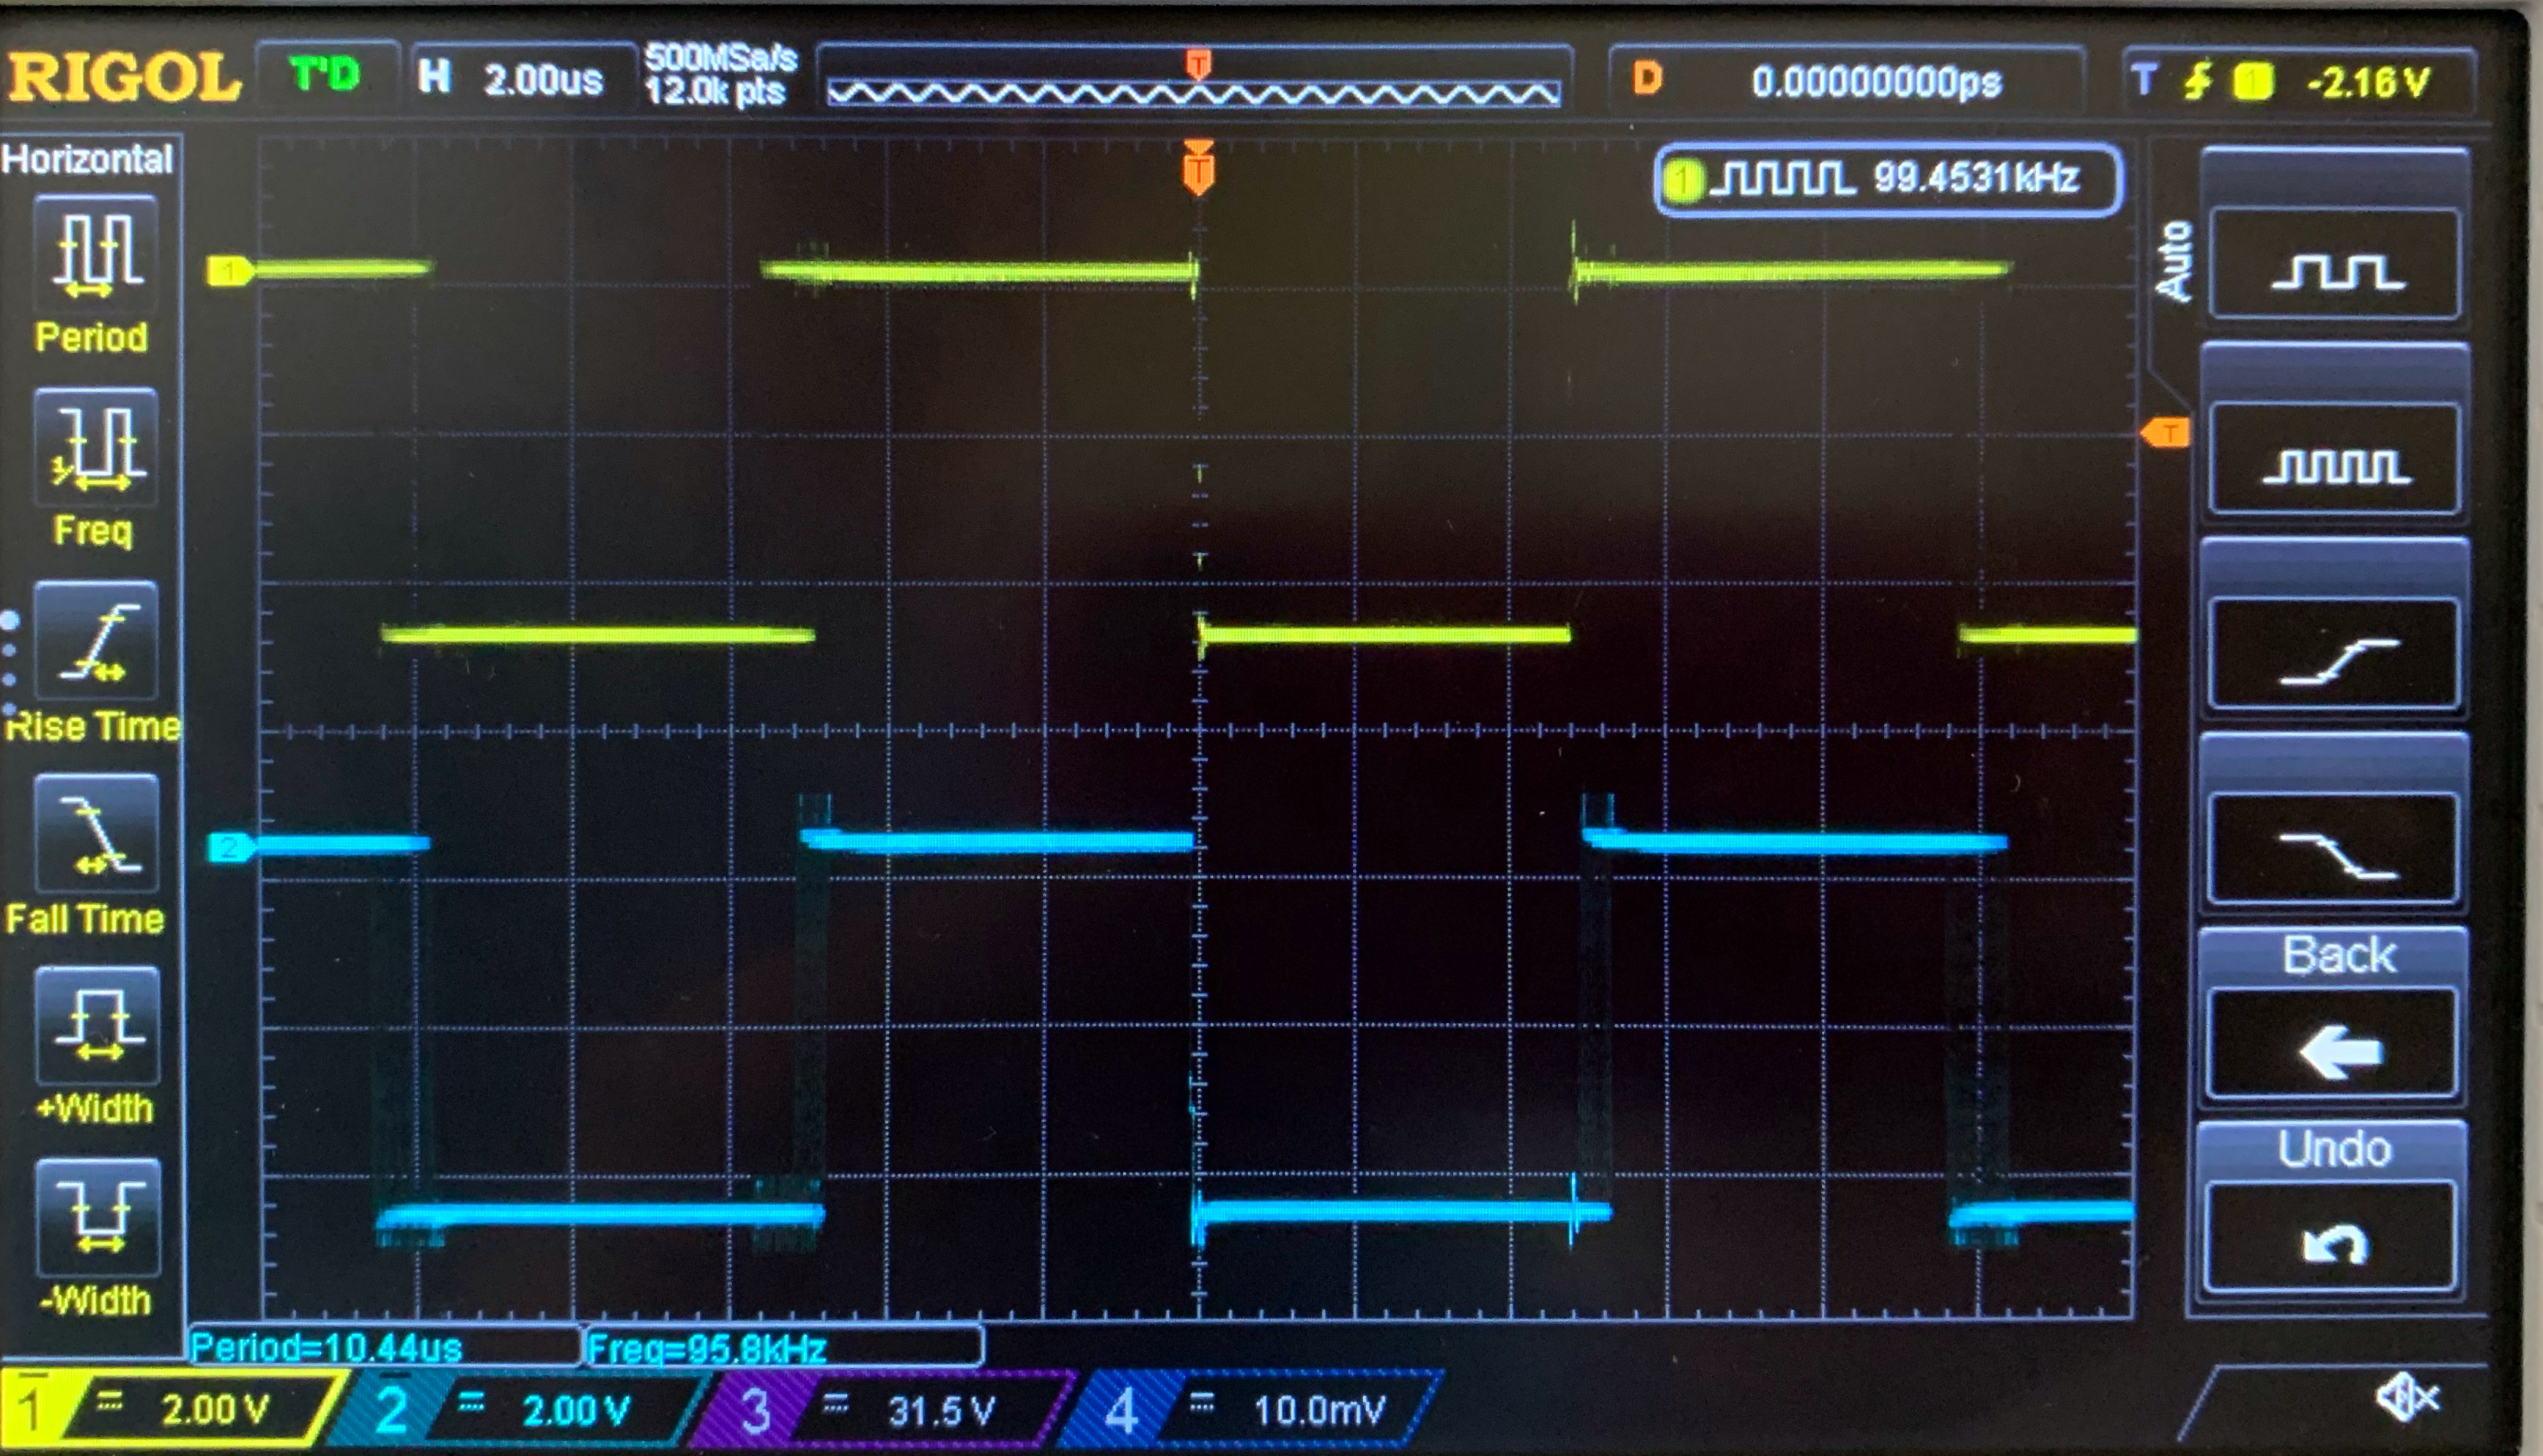
\includegraphics[width=15cm]{W3Q5a_.jpg}
    \caption{Pulse width of the TTL signal}
    \label{fig:W3Q5a_}
\end{figure}
\item %b 
After confirming the zero crossing detector we fed our FM message ($\beta=2$) to generate the zero crossings. Figure \ref{fig:W3Q5b_a} shows the output (yellow) compared to the input FM signal (blue). 
\begin{figure}[H]
    \centering
    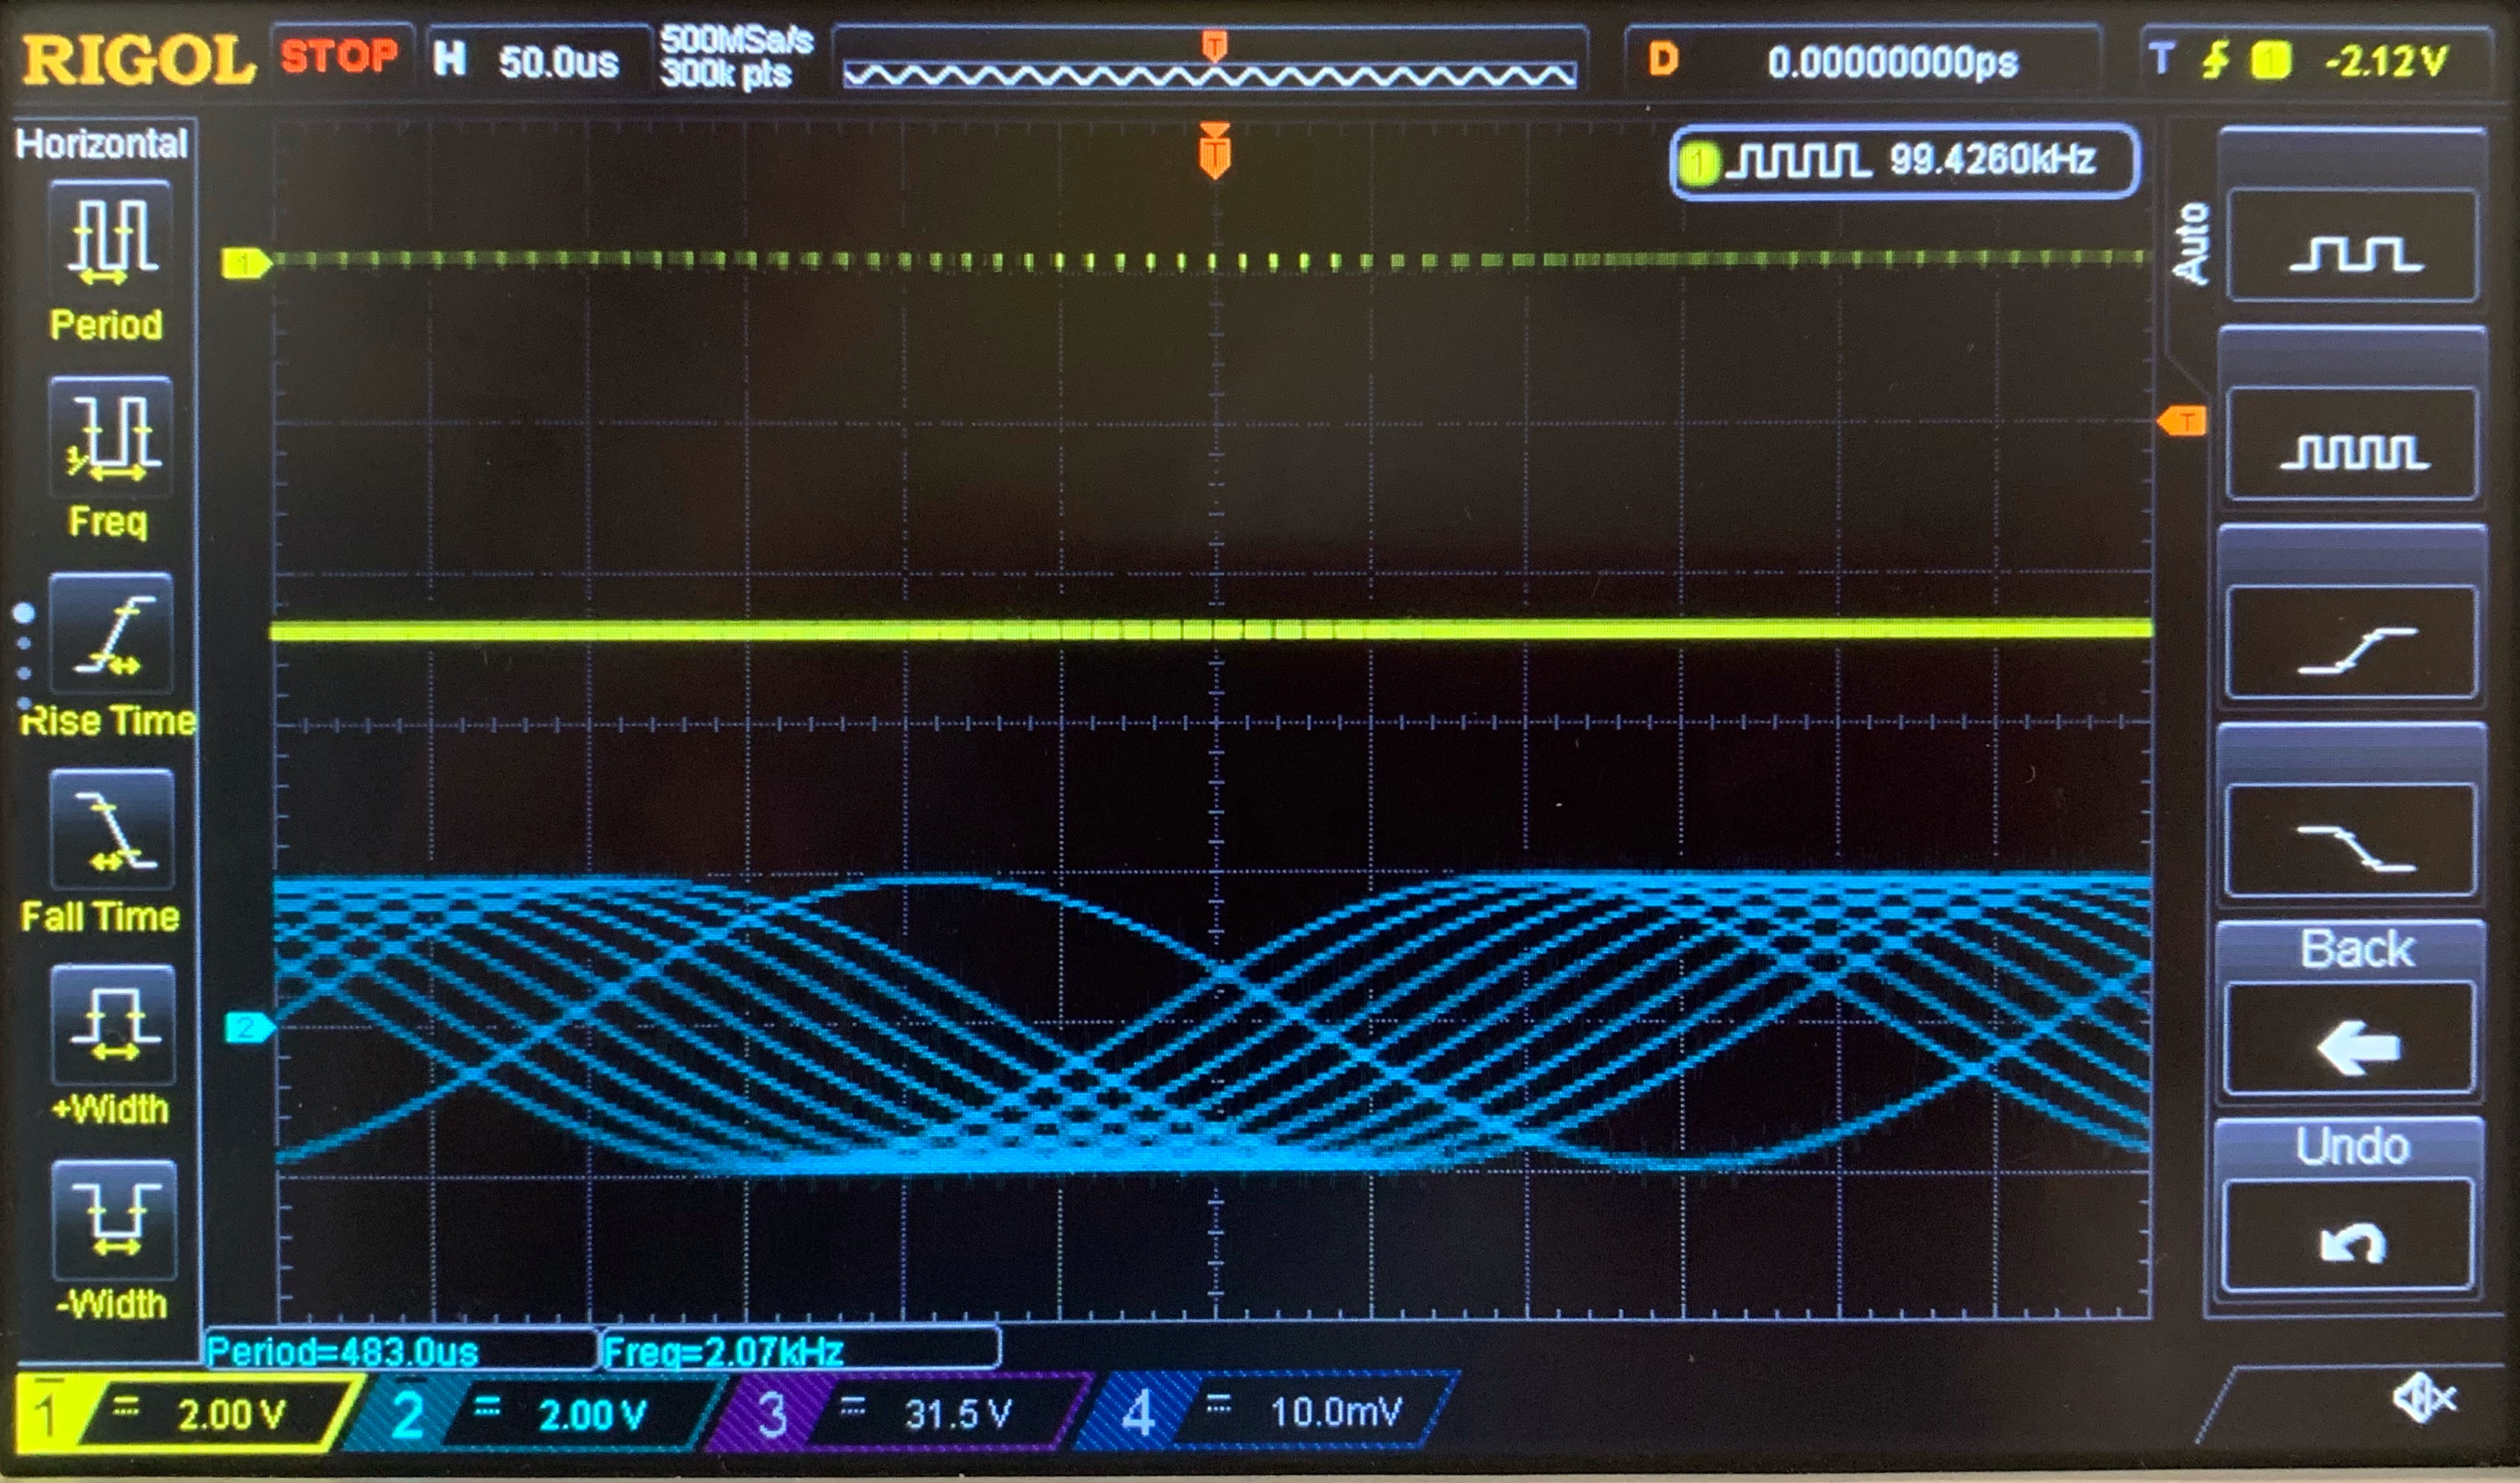
\includegraphics[width=15cm]{W3Q5b_a.jpg}
    \caption{Zero crossing detection of the FM message signal}
    \label{fig:W3Q5b_a}
\end{figure}
The pulse width because of the varying frequency would be less than 50\% of the carrier frequency pulse period of $\frac{1}{100\text{kHz}} = 10\mu$s as shown in Figure \ref{fig:W3Q5b_}. The measured pulse width of 2.52$\mu$s matches our calculations of 2.5$\mu$s, where the 2kHz message has a period of 50$\mu$s and as a percentage of the pulse period, it is significant in 5$\mu$s; 50\% of this gives the pulse width of 2.5$\mu$s.

%Insert calculations of 2kHz as a percentage of 100kHz period being 2.5us  % isn't this 2.5 us? I am not sure with this one, is this because we want to include the maximum value in the sine wave when getting zero-crossings? i.e. we include 1/4 of each period (1/100,000), which leads to a 2.5 us? 
% yea... i can't quite remember how I got here but somewhere in my scribbles I wrote something like this... 

\begin{figure}[H]
    \centering
    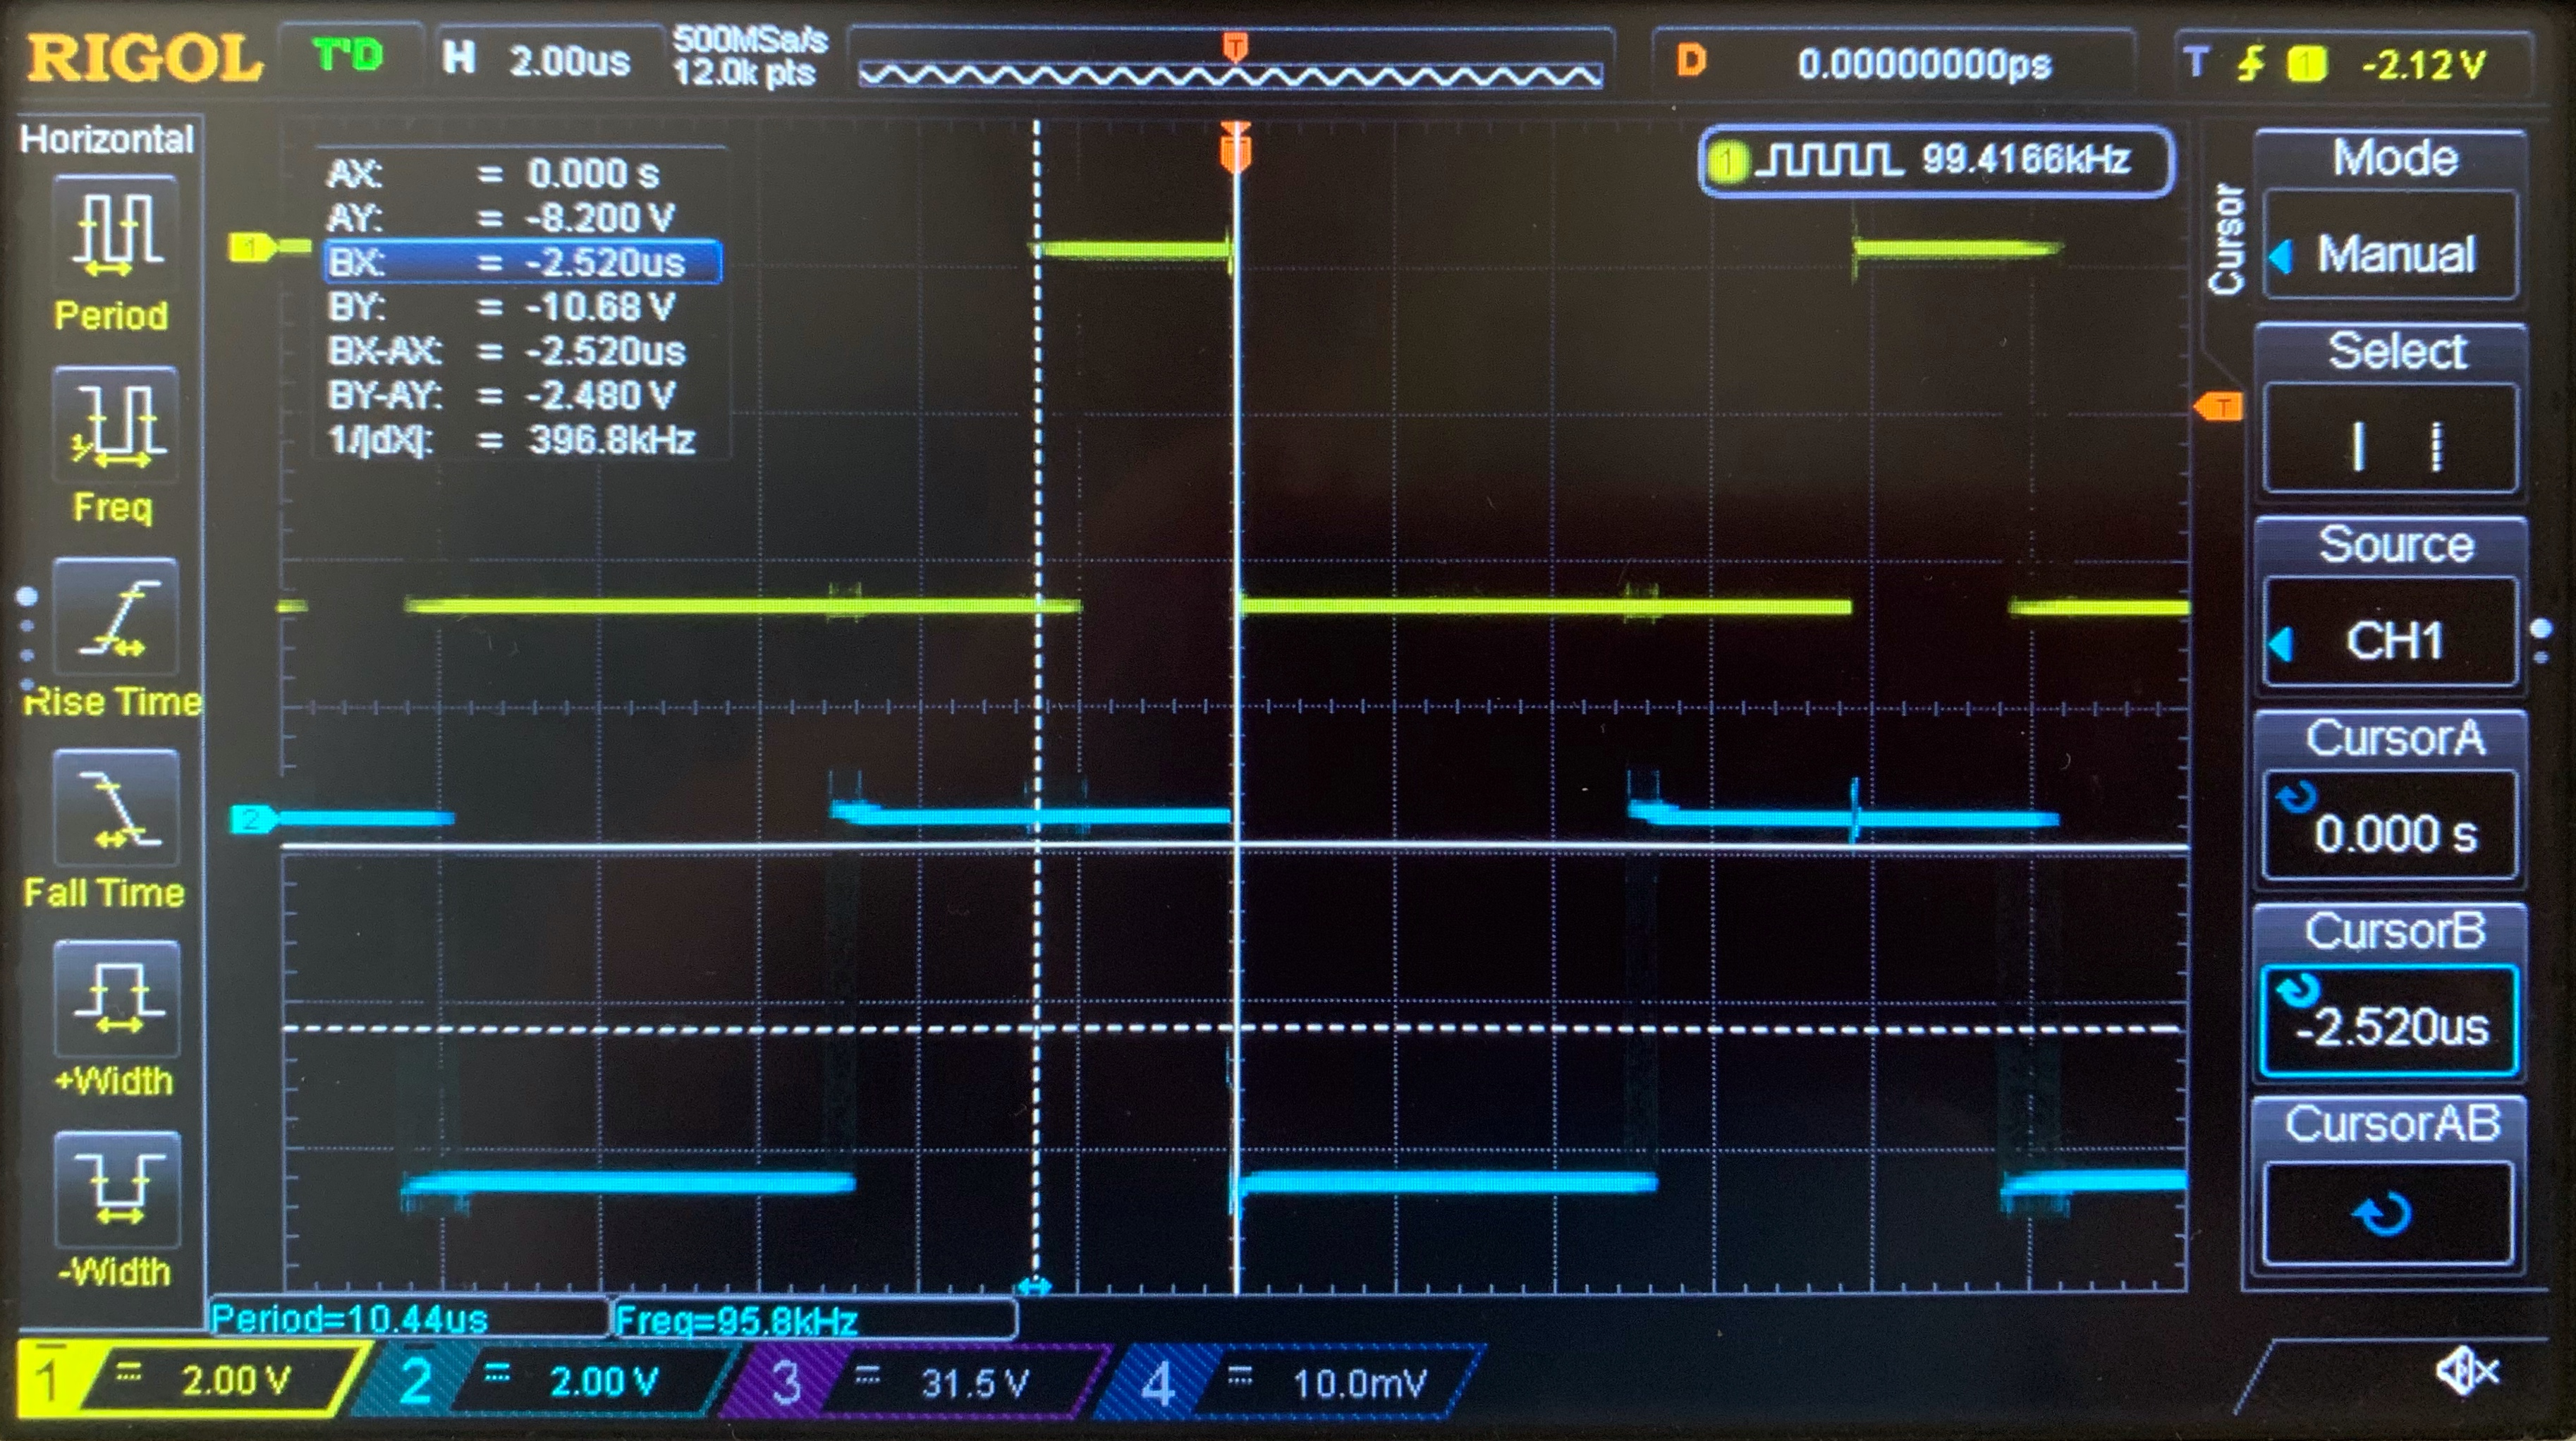
\includegraphics[width=15cm]{W3Q5b_.jpg}
    \caption{Pulse width measurement of the TTL signal from our FM message}
    \label{fig:W3Q5b_}
\end{figure}
The TTL signal is then fed through a demodulator, which is a low pass filter (LPF) that integrates across the detected zero crossings to produce the original message. The time and frequency domain outputs are shown in blue in Figure \ref{fig:W3Q5b} compared to the original 2kHz message in yellow. In spectrum, a 2kHz component can be clearly observed, which indicates a successful demodulation. 
\begin{figure}[H]
    \centering
    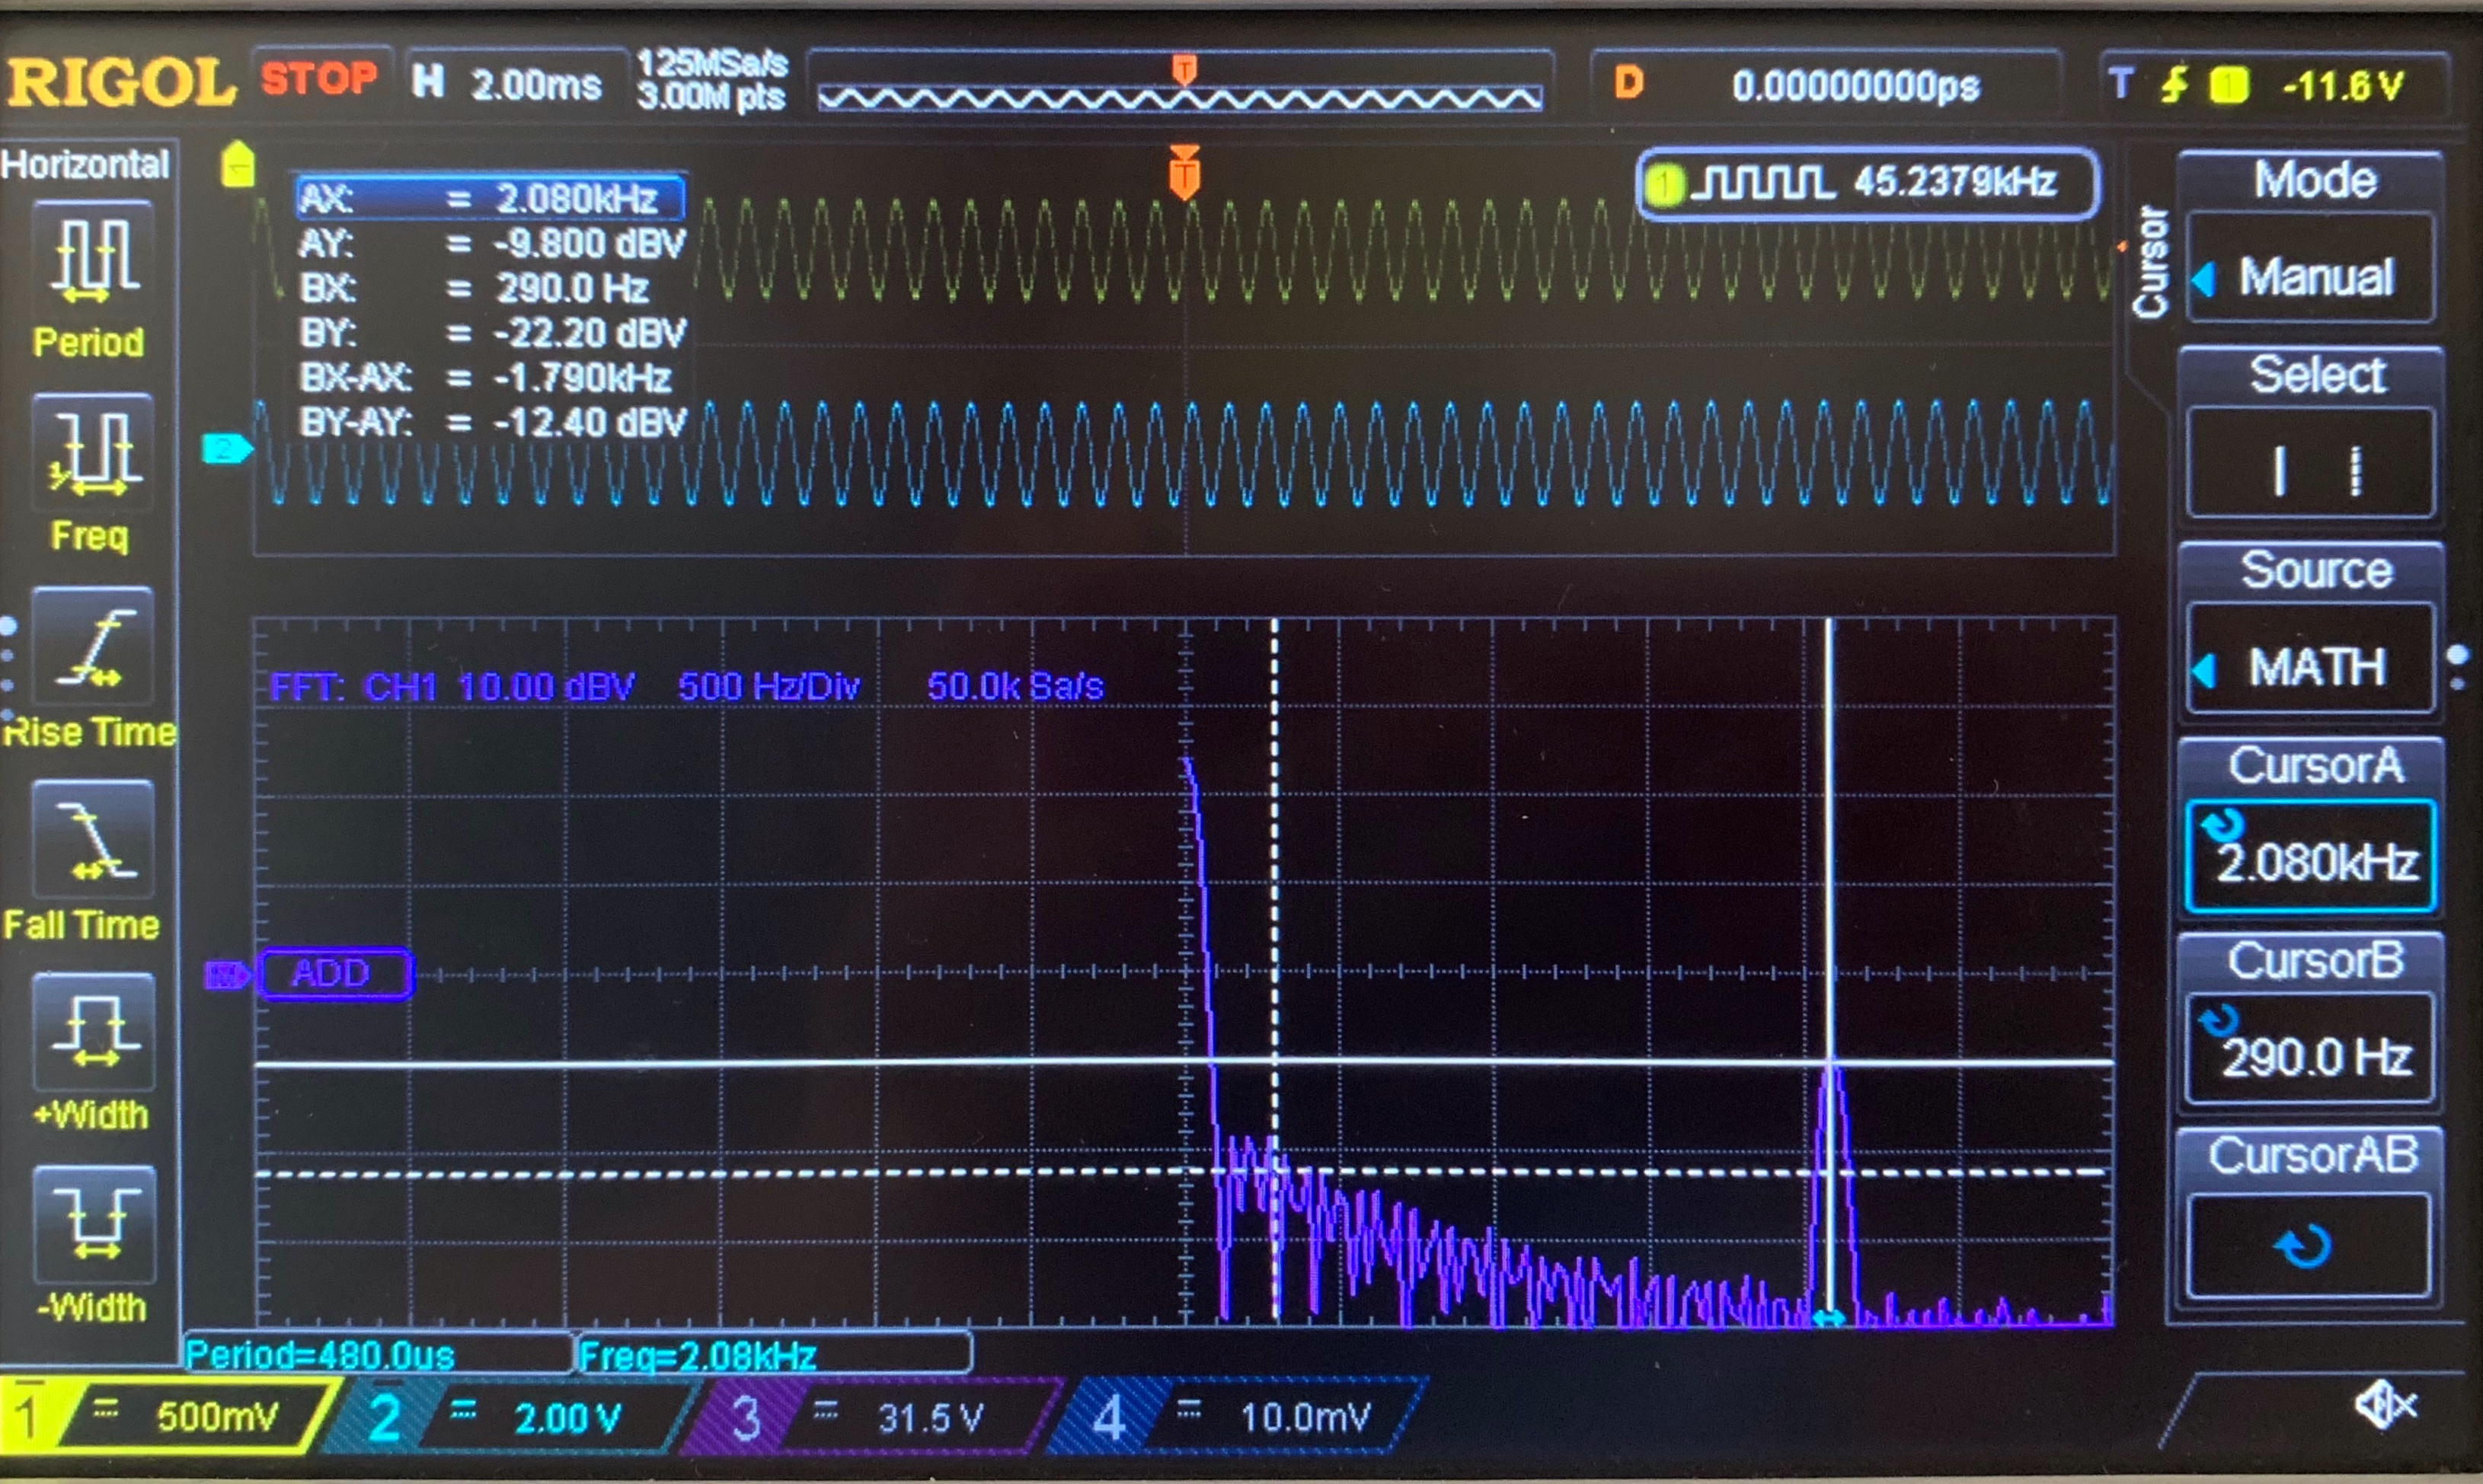
\includegraphics[width=15cm]{W3Q5b.jpg}
    \caption{Time and frequency domain representations of the 2kHz message signal after ZX signal demodulation}
    \label{fig:W3Q5b}
\end{figure}
\end{enumerate}

\subsection*{Configuration Sketch}
\begin{figure}[H]
    \centering
    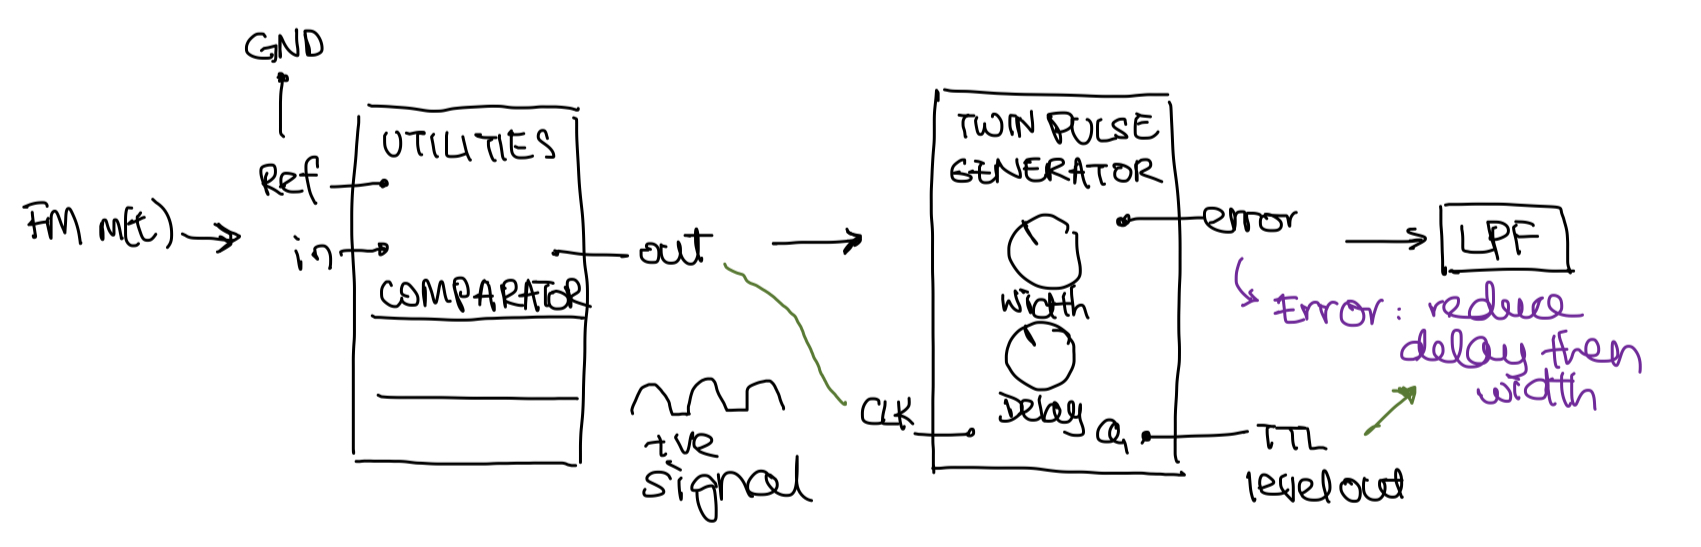
\includegraphics[width=15cm]{W3Q5Config.jpeg}
    \caption{Configuration sketch of the TTL module and ZX detector}
    \label{fig:W3Q5Config}
\end{figure}

\newpage
\section*{Question 6}
\begin{enumerate}[label=(\alph*)]
\item %a
Our demonstrator has checked the 100kHz output of both VCOs in free run. See attached sign offs. 
\item %b
Refering to our circuit setup in Figure \ref{fig:W3Q6Config} the received FM signal $x(t)$ that we are feeding through the phase locked loop (PLL) is $x_{FM}(t) = A_c \cos(2\pi f_c t + 2\pi k_f \int^t_0 m(\tau) d\tau)$. 
The output $y(t)$ fed through the VCO is $y_{VCO}(t) = -\sin(2\pi f_v t + 2\pi k_v \int^t_0 y(\tau)d\tau)$. When multiplied we have the following, 
\begin{align*}
    x'(t) &= -A_c \cos(2\pi f_c t + 2\pi k_f \int^t_0 m(\tau) d\tau) \sin(2\pi f_v t + 2\pi k_v \int^t_0 y(\tau)d\tau)\\
    &= -A_c \cos(\theta_c) \sin(\theta_v)\\
    &= -\frac{A_c}{2} \bigg[ \sin(\theta_v - \theta_c) - \sin(\theta_v + \theta_c) \bigg]
\end{align*}
where $\theta_c = 2\pi f_c t + 2\pi k_f \int^t_0 m(\tau) d\tau$ and $\theta_v = 2\pi f_v t + 2\pi k_v \int^t_0 y(\tau) d\tau$.\\
Passing the above through a LPF we remove the second high frequency term. And the remaining output $y(t)$ needs only the PLL gain $K_a$ added. The final output is expressed as,
\begin{align*}
    y(t) &= \frac{A_c}{2} K_a \sin(\theta_c - \theta_v) \approx \frac{A_c}{2} K_a \epsilon(t)
\end{align*}
We aim to keep the angle difference $\epsilon(t) = \theta_c - \theta_v$ small so that the circuit is phase locked. Expanding and rearranging $\epsilon(t)$ we have the following ODE, 
\begin{align*}
    \frac{d\epsilon(t)}{dt} &= 2\pi(f_c - f_v) + 2\pi[k_f m(t) - k_v y(t)]\\
    &= 2\pi(f_c - f_v) + 2\pi[k_f m(t) - \frac{A_c}{2} k_v K_a \sin(\epsilon(t))]\\
    &\approx 2\pi(f_c - f_v) + 2\pi[k_f m(t) - \frac{A_c}{2} k_v K_a \epsilon(t)]
\end{align*}
where, $\sin\epsilon(t)$ is assumed to be small so that it can be approximated as $\epsilon(t)$.\\ 
The Fourier transform of the ODE is, 
\begin{align*}
    j2\pi E(f) &= 2\pi(f_c - f_v)\delta(f) + 2\pi[k_f M(f) - \frac{A_c}{2} k_v K_a E(f)]\\
    E(f) &= \frac{(f_c - f_v)\delta(f) + k_f M(f)}{\frac{A_c}{2} k_v K_a + j\pi} \approx \frac{(f_c - f_v)\delta(f) + k_f M(f)}{\frac{A_c}{2} k_v K_a}
\end{align*}
Letting $B_L = \frac{A_c}{2} k_v K_a$, which is much larger than $j\pi$; this is the phase loop bandwidth and has the relationship $B_L >> W >> f$. The angle difference can now be expressed as a DC term and a frequency demodulation term, 
\begin{align*}
    \epsilon(t) &= \frac{(f_c - f_v)}{B_L} + \frac{k_f m(t)}{B_L}
\end{align*}
Substituting this back into $y(t)$ gives us, 
\begin{align*}
    y(t) &= \frac{A_c}{2} K_a \bigg[\frac{(f_c - f_v)}{B_L} + \frac{k_f m(t)}{B_L}\bigg] = \frac{(f_c - f_v)}{k_v} + \frac{k_f m(t)}{k_v}
\end{align*}
To avoid distortion, the DC term should be kept to a minimum and hence aiming for $\Delta f = f_c - f_v = 0$. Zero isn't practically possible so the practical aim is to keep $\Delta f << B_L$. To get the output $y(t)$ as close to $m(t)$ i.e. reducing $\epsilon(t)$, $\frac{k_f|m(t)|_{max}}{k_v}$ should be $\leq 1$.\\
Using our FM message signal of $\beta = 2$ at $k_f = 13.2$ for this exercise, $A_m = |m(t)|_{max}$ was set to 0.3V. This gives the inequality $k_v \geq 3.96$.

%The PPL sensitivity should maintain that $W<< 0.5 k_v k_a A_c$ for minimal distortions, which leads to $2<< 0.5 k_v k_a \times 2.5$. We assume $0.5 k_v k_a \times 2.5$ to be 10 times larger than $W$, we will have $k_v>\frac{16}{k_a}$. Therefore, the range of $k_v$ should depend on the choice of $k_a$ in PPL. 

% some value that doesn't go through overlap... enter calculations

%Ac = 2.5V amplitude not Vpp
% I wrote down a bunch of stuff saying Vpp 1.52/1.54V and 4.24 original with Am 0.270V? not too sure what this is in relevance to 

% I think we use W << 0.5 k_v K_a A_c (see p8,L11) ? Where K_a is the gain we adjusted, A_c is the magnitude of the modulated signal (equal to mag of carrier, see if you have it, I didn't note down), W is message bandwidth (frequency f_m=2kHz), and we have k_f = 13.2 . So we should be able to get a lower bound of K_v. This might be useful for sub-Q d) as well. Not sure if there is any upper bound. Not been mentioned in the lecture notes. I do remember we had adjusted the gain to get the output waveform to be correct. So regarding Q6, there should be a lower bound came from experiments. We might didn't note it down.

\item %c
Figure \ref{fig:W3Q6b} shows the PLL demodulated signal in yellow in comparison with the original 2kHz message in blue. The FFT shows a clear peak at 2kHz indicating a successful demodulation. %From the peak half way from the 2kHz position, the PLL VCO gain seems to be set at 0.5.

% idk, actually i dont think it asks for the gain. the time-domain waveform is not in dB. only fft is.  %%% hmmmm I'm not sure that it's 0.5 in time domain though, sorry I thought you were talking about the side peak. Because the scale on yellow is 5V/unit and blue is 2V/unit... I don't think they're comparable in this view? Commented that out... 


\begin{figure}[H]
    \centering
    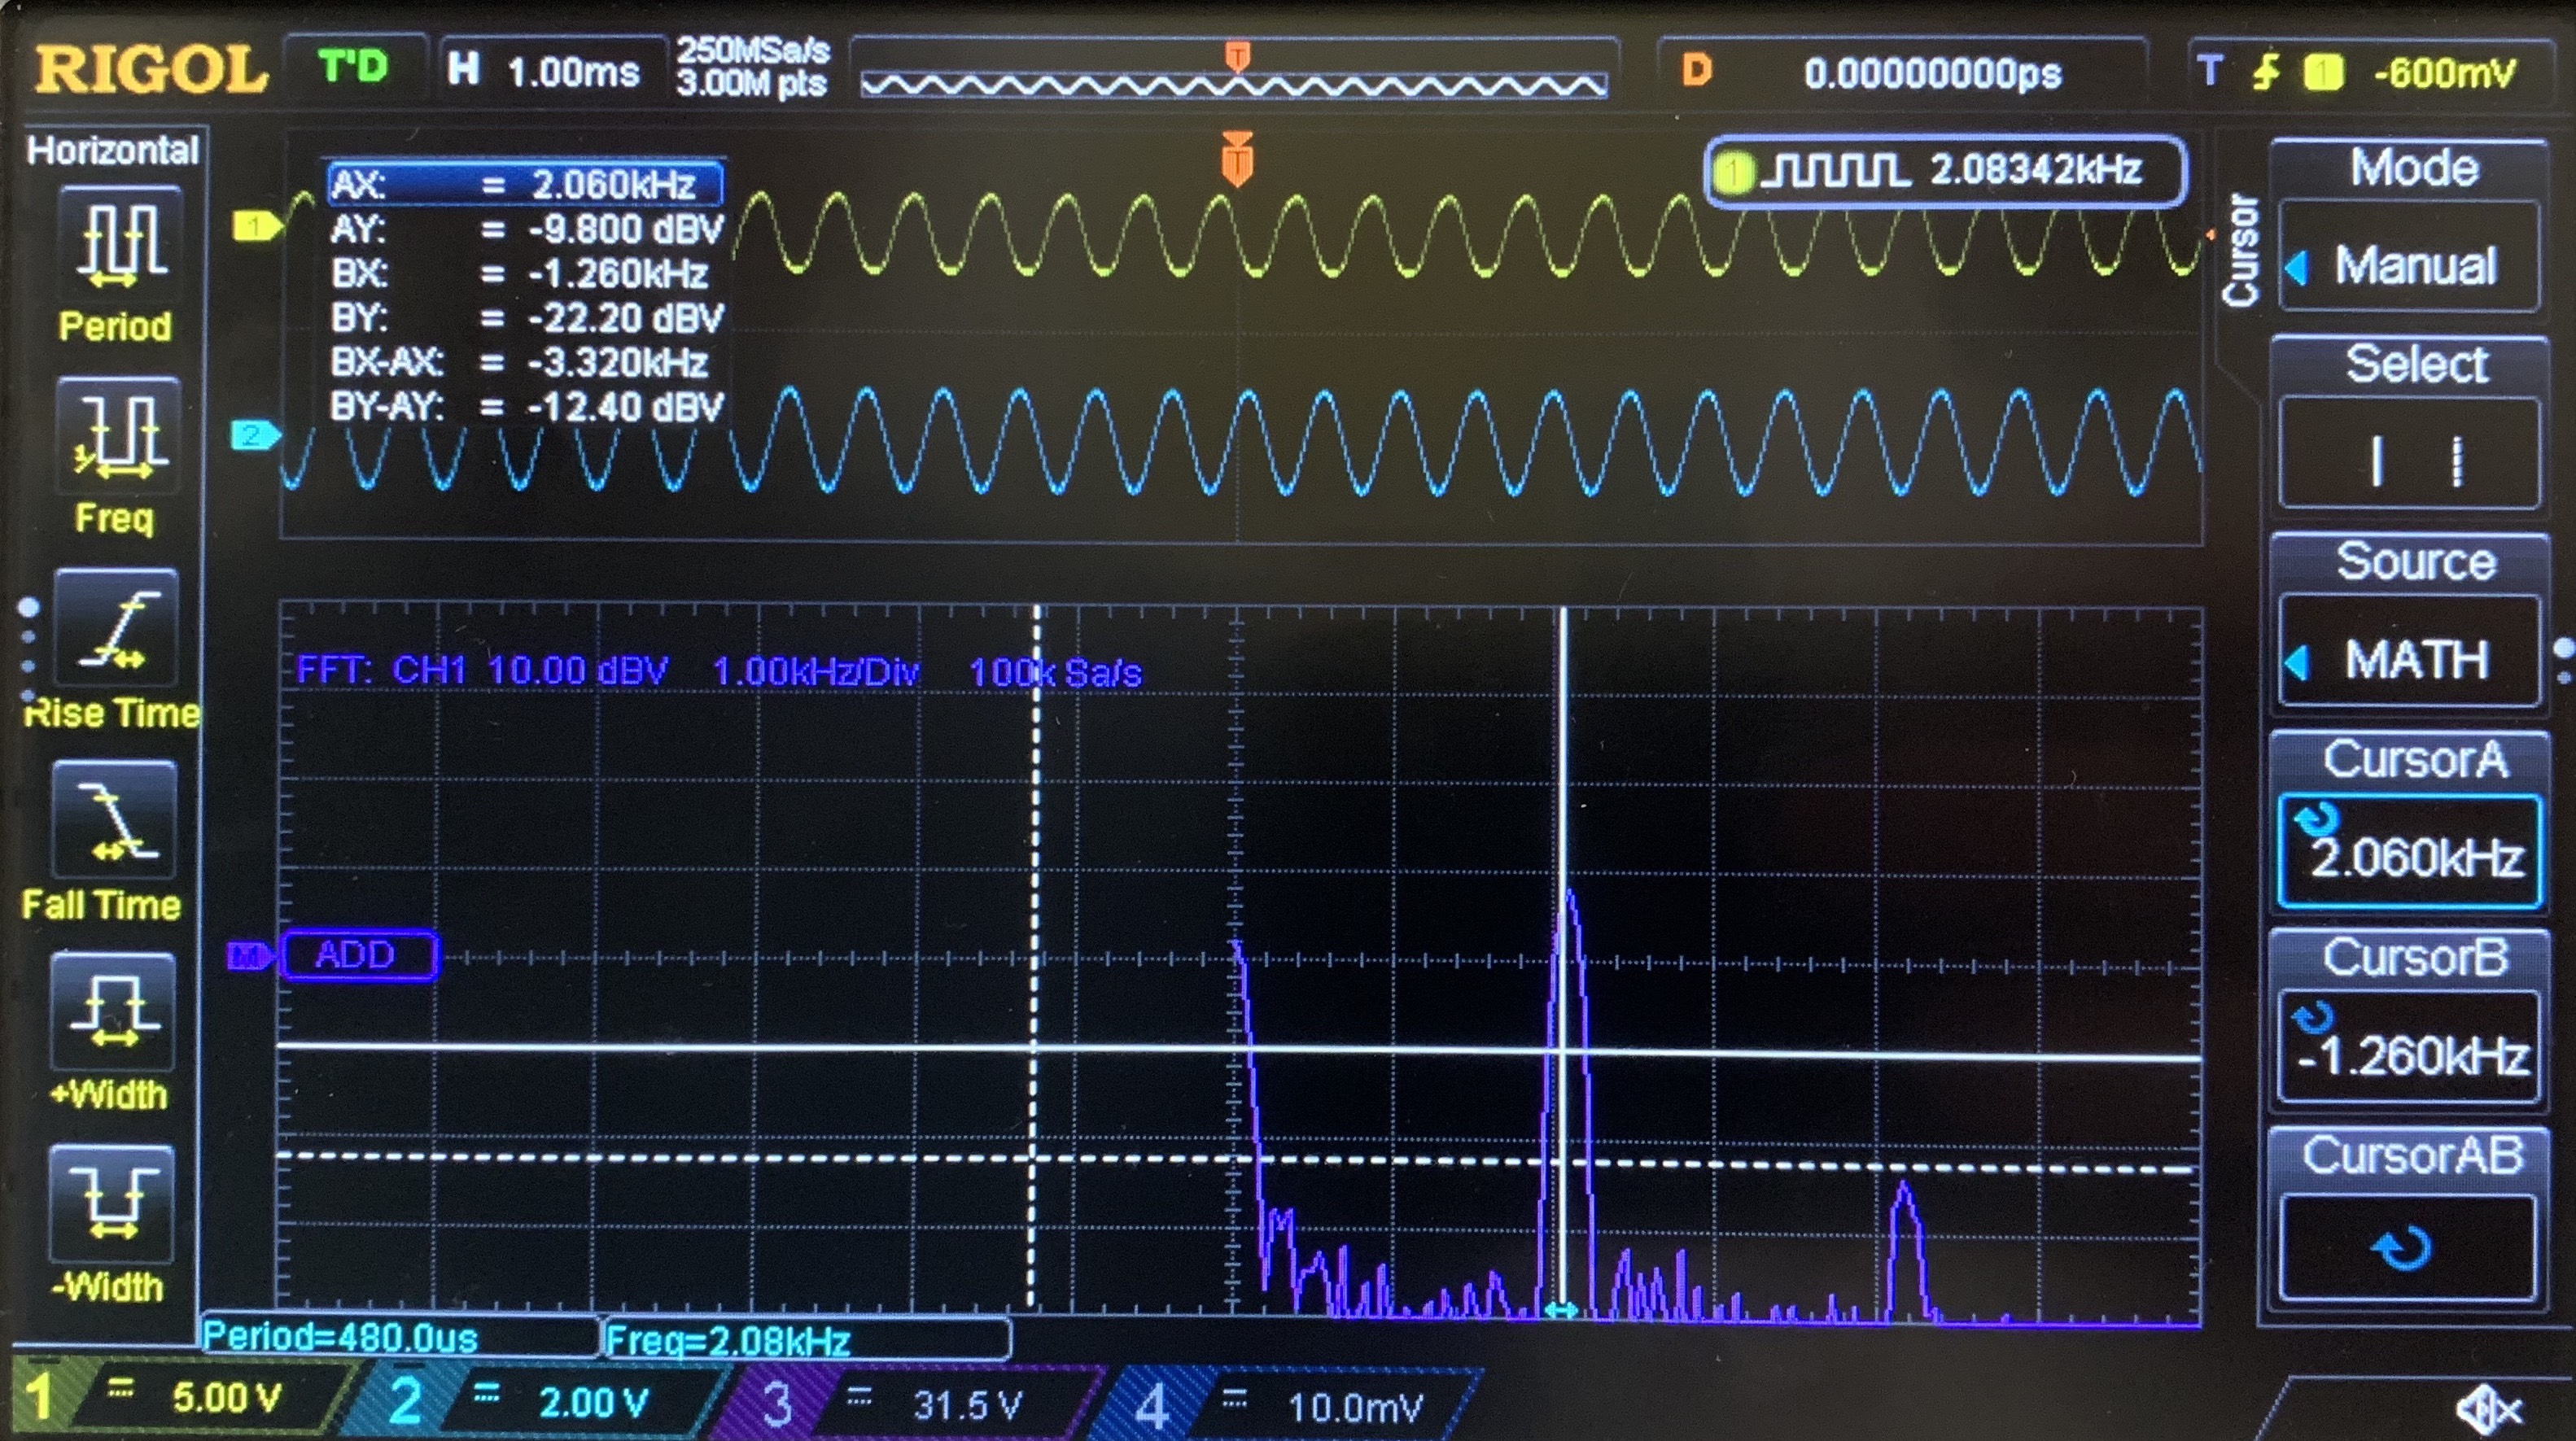
\includegraphics[width=15cm]{W3Q6b.jpeg}
    \caption{PLL demodulated signal in time and frequency domains}
    \label{fig:W3Q6b}
\end{figure}

\item %d
% do we have the values of kv in the following graphs? we'd better to say something about the lowest kv we had to maintain no distortions.. It might be hard, it slipped my mind in the workshop.

% No we didn't have kv values coz it was too hard to measure the exact value unless we measured the amplitudes again... 

% thats fine then, lets just leave it like this.

We tuned the VCO gain controlling the PLL part of the demodulator and captured the following output in Figure \ref{fig:W3Q6b_}. From the FFT we see more than a single peak, which shows that additional frequencies are present and we see this in the output in yellow that deviates significantly from the original signal (blue).
\begin{figure}[H]
    \centering
    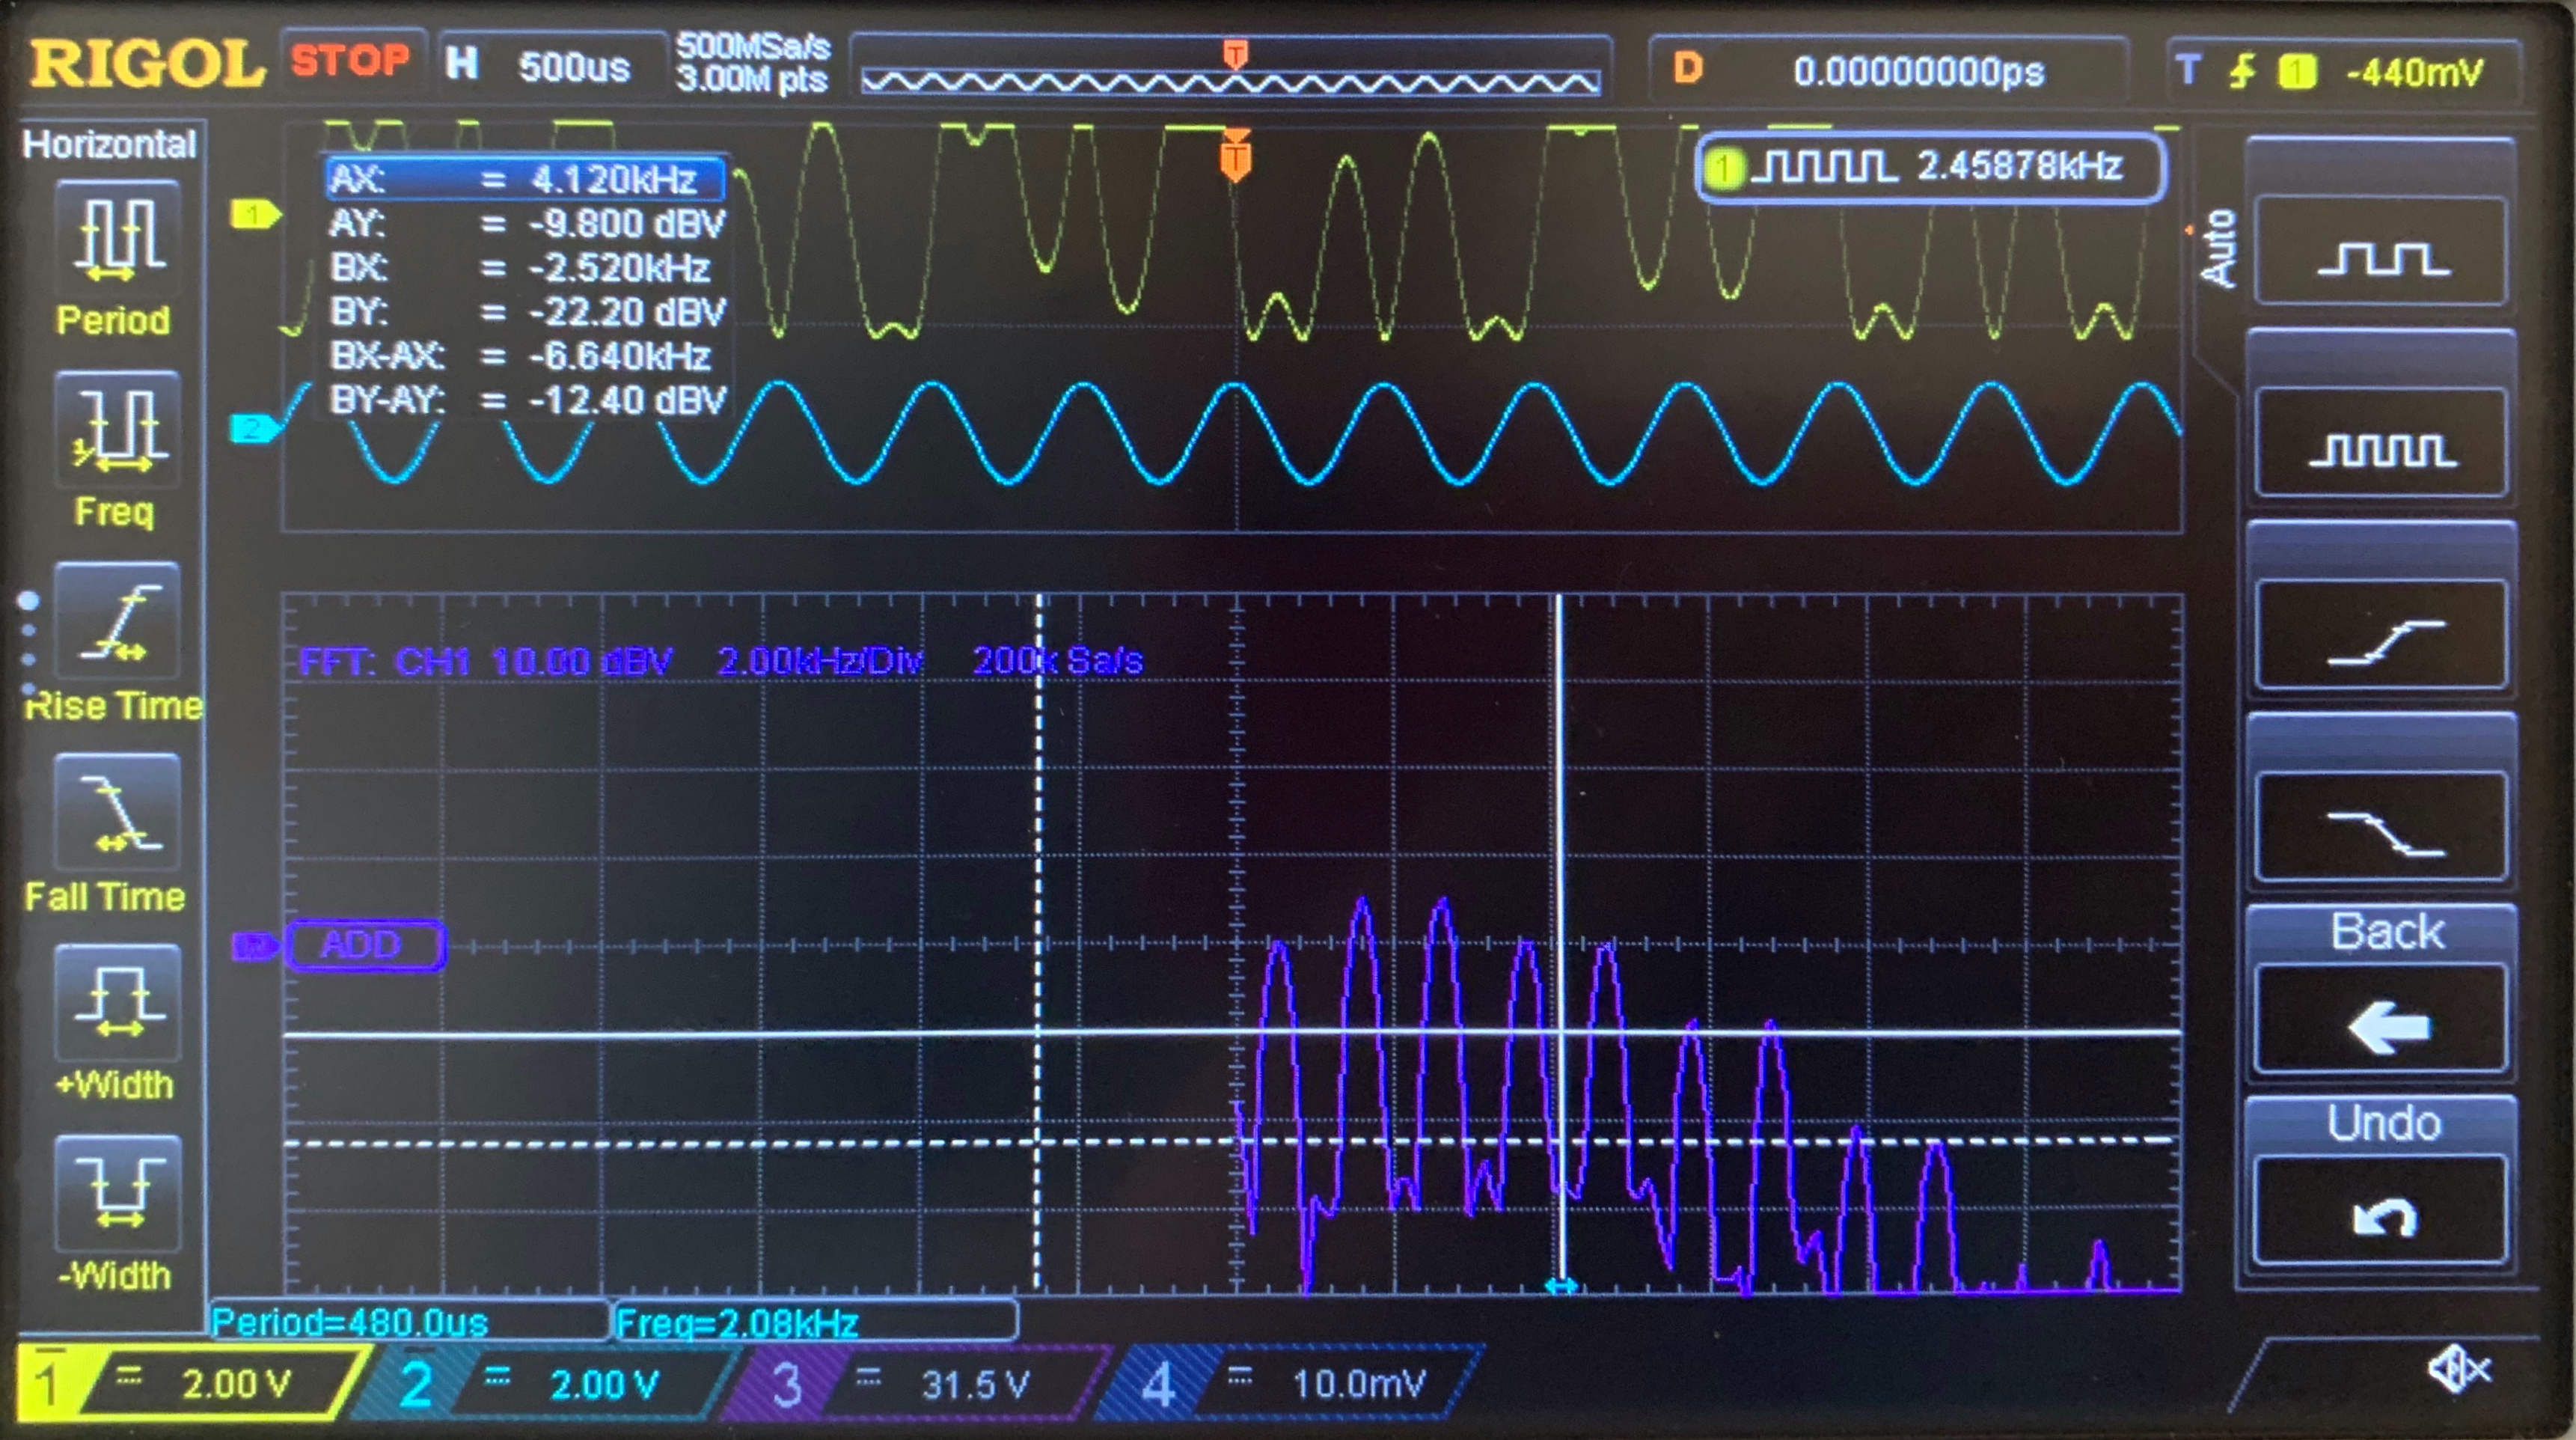
\includegraphics[width=15cm]{W3Q6b_.jpg}
    \caption{PLL demodulated signal with adjusted higher $k_v$}
    \label{fig:W3Q6b_}
\end{figure}
Further tuning the VCO gain, we also get Figure \ref{fig:W3Q6b_a}. The FFT shows a lower than 2kHz peak. We see the output in yellow have a similar shape to the original signal with additional oscillations in between due to the lower frequencies.
\begin{figure}[H]
    \centering
    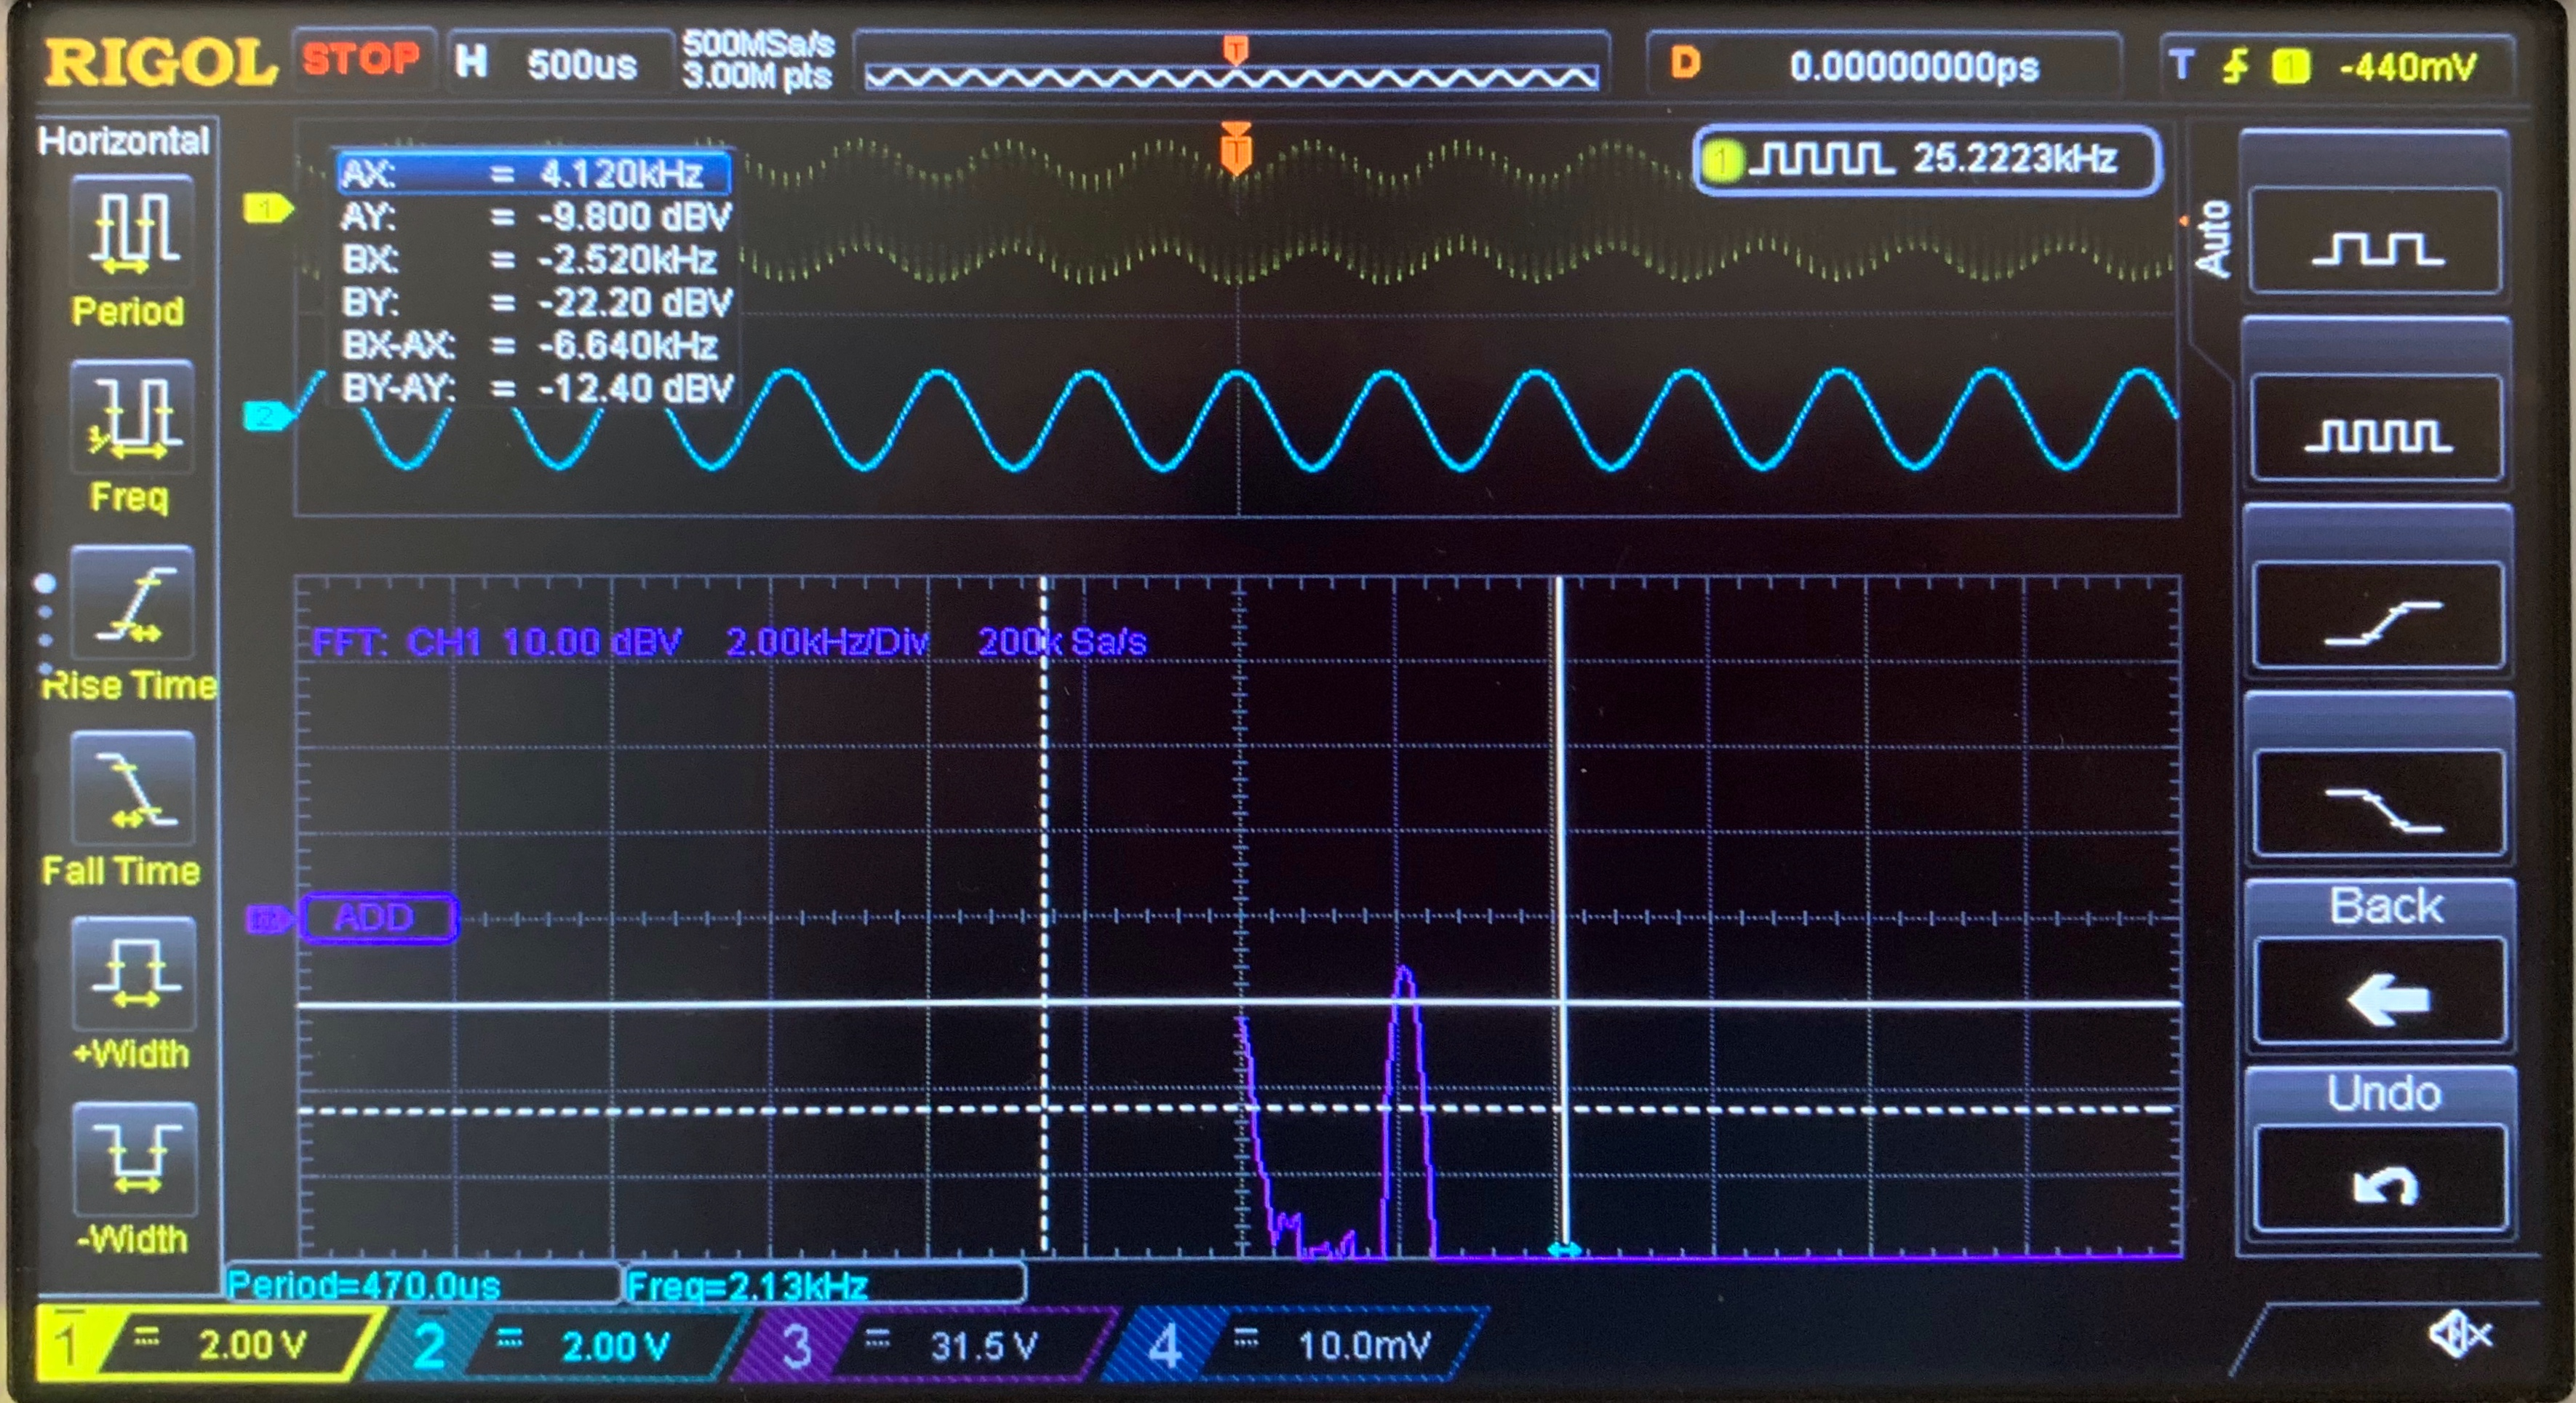
\includegraphics[width=15cm]{W3Q6b_a.jpg}
    \caption{PLL demodulated signal with adjusted lower $k_v$}
    \label{fig:W3Q6b_a}
\end{figure}
For the above, when we tuned the second VCO gain we could not precisely measure $k_v$'s value as it was an analog dial. We tuned the $k_v$ with the purpose of seeing the effects of out of bound values. 
\end{enumerate}

\subsection*{Configuration Sketch}
\begin{figure}[H]
    \centering
    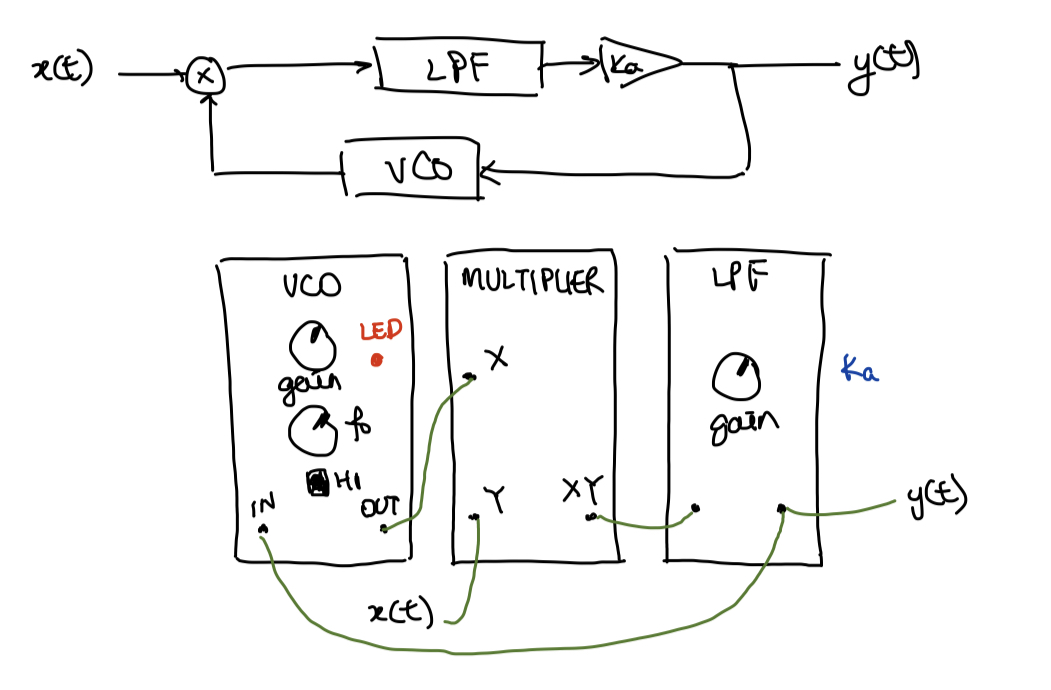
\includegraphics[width=10cm]{W3Q6Config.jpeg}
    \caption{Configuration sketch of the VCO and LPF setup of a PLL}
    \label{fig:W3Q6Config}
\end{figure}

\section*{Appendix: Check-offs}
Please kindly find check-offs on the following pages.
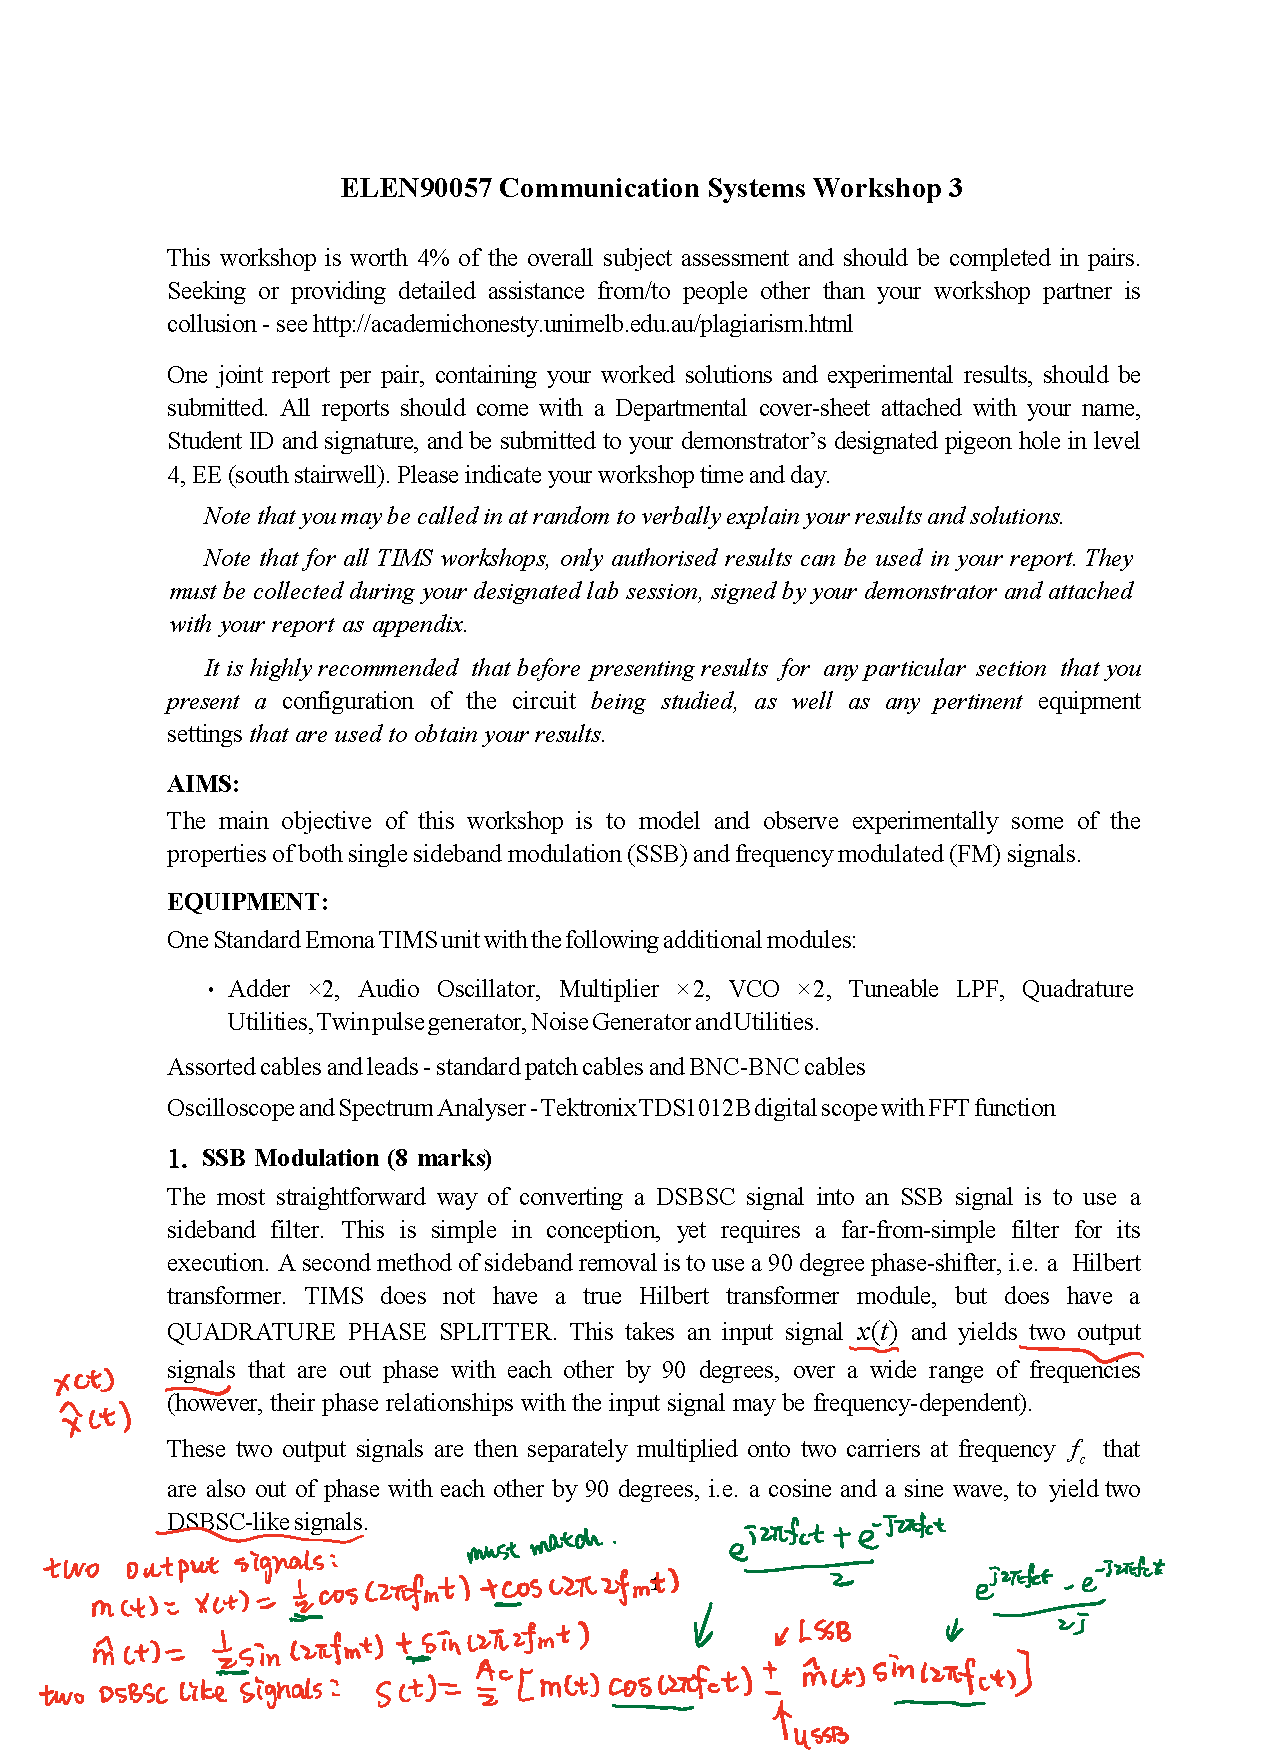
\includepdf[pages={1,3-7},scale=1]{WS3.pdf}
\end{document}
